% !TeX root = ../proyecto.tex

\chapter{Resultados y Análisis}\label{ch:resultados-y-analisis}
En este capítulo se exponen los experimentos realizados y los resultados obtenidos en los distintos escenarios evaluados.
El objetivo principal fue analizar el rendimiento de los modelos entrenados con conjuntos de datos reducidos,
seleccionados mediante los distintos algoritmos desarrollados a lo largo del proyecto.



\section{Resultados con el conjunto completo}\label{sec:resultados-conjunto-completo}
Como punto de partida, se evalúa el rendimiento de los modelos convolucionales entrenados con el \textbf{100\%} del conjunto de datos.
Esta prueba sirve como referencia para contrastar los resultados obtenidos mediante las técnicas de reducción aplicadas posteriormente.
Se emplean los modelos \textbf{ResNet50} y \textbf{MobileNetV2}, y se miden las métricas de \textit{accuracy},
\textit{precision}, \textit{recall} y \textit{F1-score} sobre el conjunto de validación.

\begin{table}[htp]
    \centering
    \resizebox{\textwidth}{!}{
        \begin{tabular}{P{2cm} P{2.5cm} P{2.5cm} P{2.5cm} P{2cm}}
            \toprule
            \textbf{Duración por Eval.} & \textbf{Accuracy (Avg)} & \textbf{Precision (Avg)} & \textbf{Recall (Avg)} & \textbf{F1-score (Avg)} \\
            \midrule
            \multicolumn{5}{l}{\textbf{Modelo ResNet50}}                                                                                       \\
            \midrule
            00:02:42                    & 87,90\%                 & 88,96\%                  & 87,90\%               & 87,81\%                 \\
            \midrule
            \multicolumn{5}{l}{\textbf{Modelo MobileNet}}                                                                                      \\
            \midrule
            00:03:16                    & 78,60\%                 & 81,55\%                  & 78,60\%               & 77,68\%                 \\
            \bottomrule
        \end{tabular}
    }
    \caption{Comparativa de resultados del \textbf{100\%} con los modelos \textbf{ResNet50} y \textbf{MobileNet}.}
    \label{tab:resultados-100-resnet50-mobilenet}
\end{table}

\begin{figure}[htp]
    \centering
    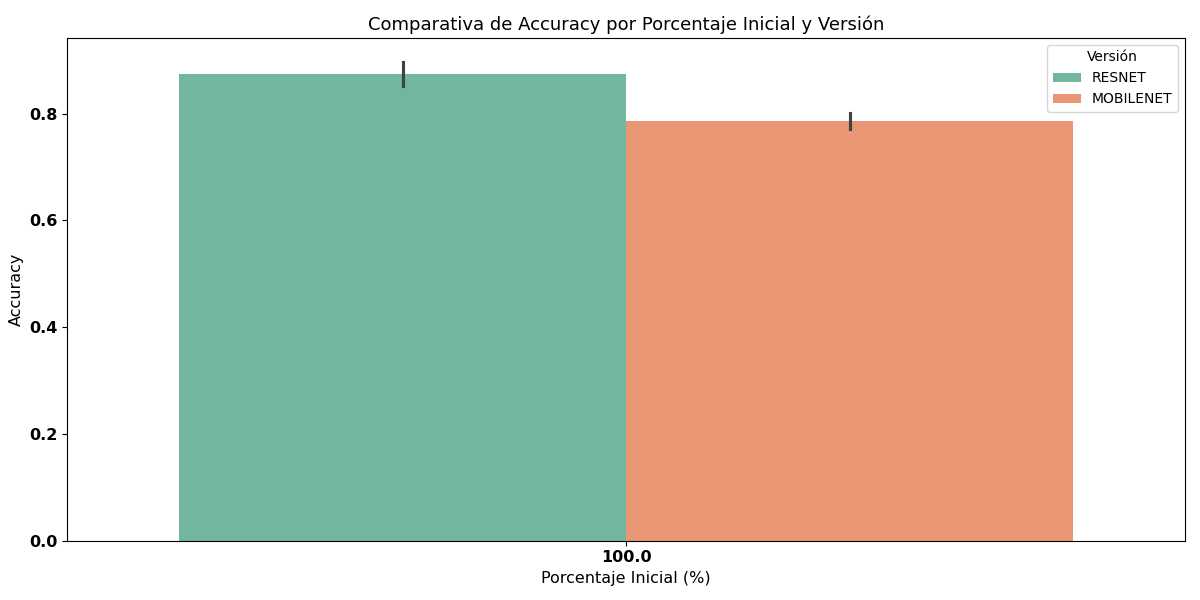
\includegraphics[width=0.95\textwidth]{imagenes/evaluaciones/comparacion_modelos_100}
    \caption{Comparación de \textit{accuracy} de los modelos ResNet50 y MobileNetV2 usando el 100\% del conjunto de datos.}
    \label{fig:comparacion_modelos_100}
\end{figure}

Los resultados presentados en la tabla~\ref{tab:resultados-100-resnet50-mobilenet}, y visualizados en la figura~\ref{fig:comparacion_modelos_100},
representan el rendimiento máximo alcanzable en condiciones ideales,
es decir, utilizando la totalidad del conjunto de datos sin aplicar técnicas de reducción.
Este escenario establece un techo de rendimiento que se utiliza como referencia para evaluar la eficacia de
los algoritmos de reducción de datos implementados en el resto del estudio.

En particular, se observa que \textbf{ResNet50} obtiene mejores resultados en todas las métricas evaluadas,
destacando especialmente en \textit{accuracy} y \textit{precision}, donde supera por más de 9 puntos porcentuales a \textbf{MobileNetV2}.
Esta superioridad en el rendimiento viene acompañada de un tiempo por evaluación ligeramente menor (\textbf{00:02:42} frente a \textbf{00:03:16}),
lo que indica una mayor eficiencia en la etapa de predicción.

Esta comparativa inicial permite establecer las bases para el análisis de los resultados obtenidos mediante las técnicas de reducción de datos,
sirviendo como referencia para valorar el impacto de las estrategias aplicadas en las secciones posteriores.


\section{Comparativa inicial de modelos}\label{sec:comparativa-inicial-modelos}
Antes de aplicar los algoritmos propuestos de reducción de datos, se considera fundamental realizar una comparativa inicial entre distintos
modelos de redes neuronales convolucionales para determinar cuál de ellos es el más adecuado para los experimentos.
Esta comparación permite identificar la arquitectura que ofrece un mejor equilibrio entre rendimiento y eficiencia computacional,
estableciendo una base sólida sobre la que construir los siguientes análisis.

Para llevar a cabo esta comparativa, se utiliza el \textbf{enfoque aleatorio (RS)} como estrategia de referencia.
Al seleccionar subconjuntos de datos de manera aleatoria, sin ninguna optimización, se obtiene una línea base que permiteevaluar el
comportamiento de cada modelo en condiciones controladas.
Esta línea base es especialmente valiosa, ya que ofrece una perspectiva realista del rendimiento mínimo esperable sin aplicar técnicas
avanzadas de reducción de datos, sirviendo como punto de partida para comparar las mejoras introducidas por los algoritmos posteriores.


\begin{table}[htp]
    \centering
    \resizebox{\textwidth}{!}{
        \begin{tabular}{P{2cm} P{2.5cm} P{2.5cm} P{2.5cm} P{2cm} P{2cm} P{2cm} P{2cm}}
            \toprule
            \textbf{Porcentaje Inicial} & \textbf{Evaluaciones Realizadas} & \textbf{Duración Total} & \textbf{Duración por Eval.} &
            \textbf{Accuracy (Avg)}     & \textbf{Precision (Avg)}         & \textbf{Recall (Avg)}   & \textbf{F1-score (Avg)}                                             \\
            \midrule
            \multicolumn{8}{l}{\textbf{Modelo ResNet50}}                                                                                                                   \\
            \midrule
            10\%                        & 100                              & 01:21:37                & 00:00:48                    & 85,16\% & 86,30\% & 85,16\% & 85,02\% \\
            25\%                        & 100                              & 01:28:14                & 00:00:52                    & 87,26\% & 88,13\% & 87,26\% & 87,02\% \\
            50\%                        & 100                              & 02:27:17                & 00:01:28                    & 88,49\% & 89,51\% & 88,49\% & 88,30\% \\
            75\%                        & 100                              & 03:52:41                & 00:02:19                    & 89,89\% & 90,53\% & 89,89\% & 89,70\% \\
            100\%                       & 1                                & -                       & 00:02:55                    & 87,42\% & 88,73\% & 87,42\% & 87,18\% \\
            \midrule
            \multicolumn{8}{l}{\textbf{Modelo MobileNet}}                                                                                                                  \\
            \midrule
            10\%                        & 100                              & 00:38:16                & 00:00:22                    & 81,34\% & 82,46\% & 81,34\% & 80,52\% \\
            25\%                        & 100                              & 01:18:22                & 00:00:47                    & 80,70\% & 81,90\% & 80,70\% & 79,90\% \\
            50\%                        & 100                              & 02:26:40                & 00:01:28                    & 80,86\% & 82,65\% & 80,86\% & 80,22\% \\
            75\%                        & 100                              & 03:05:48                & 00:01:51                    & 82,26\% & 84,16\% & 82,26\% & 81,67\% \\
            100\%                       & 1                                & -                       & 00:03:16                    & 78,60\% & 81,55\% & 78,60\% & 77,68\% \\
            \bottomrule
        \end{tabular}
    }
    \caption{Comparativa de resultados de la generación inicial utilizando el \textbf{RS} y el \textbf{100\%} con los modelos \textbf{ResNet50} y \textbf{MobileNet}.}
    \label{tab:resnet50-vs-mobilenet}
\end{table}

\begin{figure}[htp]
    \centering
    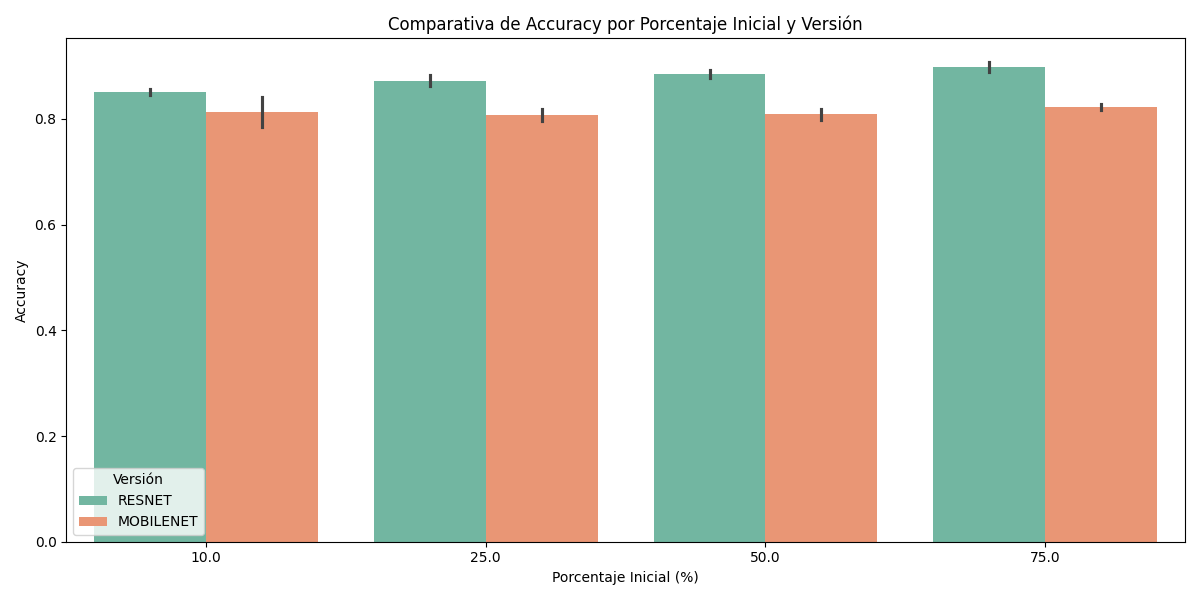
\includegraphics[width=0.95\textwidth]{imagenes/evaluaciones/comparacion_modelos}
    \caption{Diagrama de barras para comparar los modelos usando el \textit{accuracy} alcanzado por cada porcentaje inicial.}
    \label{fig:comparacion_modelos}
\end{figure}

\colorbox{yellow}{Volver a ejecutar los resultados para comprobar tiempos.}
Se realizan pruebas con distintos porcentajes iniciales de datos seleccionados aleatoriamente (10\%, 25\%, 50\%, 75\% y 100\%), utilizando tanto ResNet50 como MobileNetV2.
Los resultados obtenidos se presentan en la Tabla~\ref{tab:resnet50-vs-mobilenet}, que resume las métricas alcanzadas por cada modelo,
y en la Figura~\ref{fig:comparacion_modelos}, que muestra la comparación de los valores de \textit{accuracy} mediantes barras separados por los porcentajes iniciales.

Los resultados muestran que ResNet50 logra un mejor rendimiento en términos de \textit{accuracy}, \textit{precision}, \textit{recall} y \textit{F1-score}.
Sin embargo, este mejor rendimiento viene acompañado de un tiempo de entrenamiento considerablemente mayor.
Por su parte, MobileNetV2 ofrece una solución más eficiente en cuanto a tiempos de ejecución, a costa de una ligera pérdida de precisión,
lo que la convierte en una opción atractiva para entornos con recursos computacionales limitados.

En conjunto, esta comparativa inicial permite elegir MobileNetV2 como modelo principal para el resto de experimentos.
Aunque ResNet50 ofrece una precisión ligeramente superior, su elevado coste computacional no justifica su uso en las pruebas de reducción de datos,
donde la eficiencia es un factor clave.
Además, el uso del RS como referencia permite establecer un punto de comparación para evaluar las mejoras que los algoritmos propuestos aportarían sobre esta línea base.


\section{Resultados de la búsqueda local}\label{sec:resultados-busqueda-local}
Como se describe en el apartado correspondiente (ver \hyperref[sec:algoritmo-busqueda-local]{Sección~\ref*{sec:algoritmo-busqueda-local}}),
la búsqueda local permite mejorar progresivamente una solución inicial mediante pequeñas modificaciones guiadas por el rendimiento.
En este apartado se evalúa su efectividad como alternativa más estructurada frente al enfoque aleatorio, pero sin llegar a la complejidad de los algoritmos evolutivos.
Su inclusión busca analizar hasta qué punto una estrategia simple pero guiada puede generar subconjuntos de datos más representativos y consistentes.

\begin{figure}[htp]
    \centering
    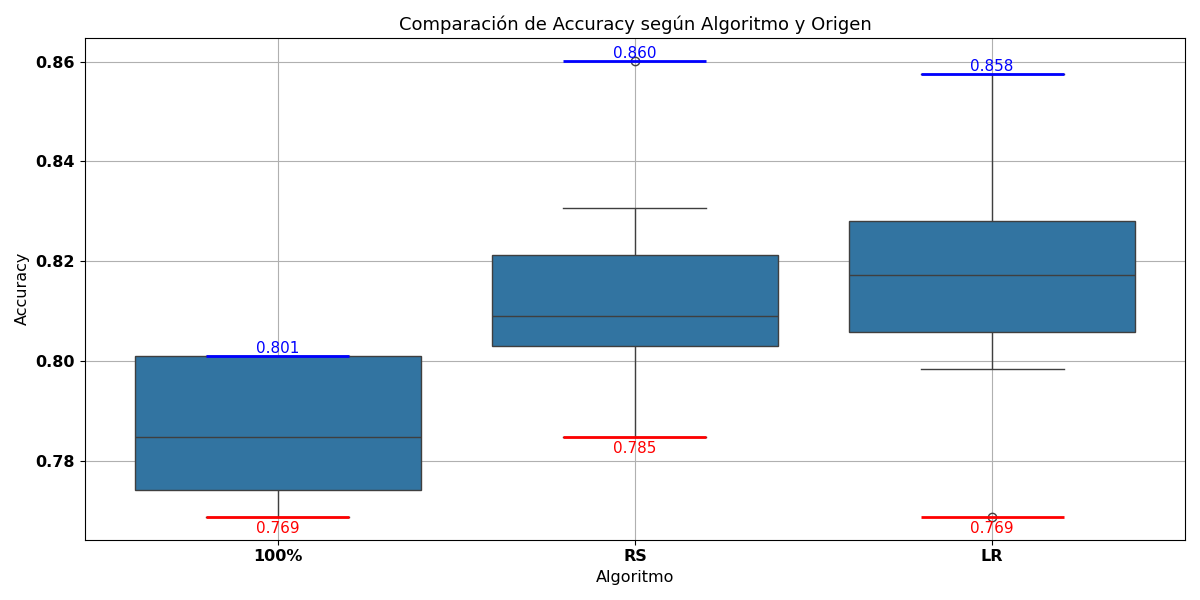
\includegraphics[width=1\textwidth]{imagenes/evaluaciones/comparacion_aleatorio-lr}
    \caption{Boxplot comparando el RS con la LS usando \textit{accuracy}.}
    \label{fig:aleatorio-vs-busqueda-local}
\end{figure}
En la Figura~\ref{fig:aleatorio-vs-busqueda-local} se muestran los resultados mediante un boxplot que permite observar
la distribución completa de valores obtenidos en las distintas ejecuciones.

Se puede apreciar que el algoritmo de búsqueda local (LS) mejora claramente la mediana del \textit{accuracy} respecto al enfoque aleatorio (RS).
Mientras que el RS se sitúa en torno a una mediana de \textbf{0.787}, la LS alcanza una mediana superior, próxima a \textbf{0.818}.
Esta diferencia refleja una mayor capacidad del algoritmo local para generar subconjuntos más representativos y eficaces.

Además, los valores máximos que alcanzan ambos algoritmos son similares (en torno a \textbf{0.858}-\textbf{0.860}),
pero la LS muestra una dispersión más acotada hacia valores altos, lo que sugiere mayor estabilidad en sus resultados.
En cambio, el RS presenta una mayor dispersión hacia valores bajos y aunque presente una mayor sensibilidad a la aleatoriedad de las selecciones,
puede llegar a tener mejores valores mínimos, como se evidencia en su menor valor mínimo (\textbf{0.785} frente a \textbf{0.769} en LS),
pero siendo el de la LS un valor atípico.

Esto pone de manifiesto que, aunque el RS puede ocasionalmente alcanzar buenos resultados,
la LS ofrece una mejor consistencia y fiabilidad, con menos varianza entre ejecuciones y una tendencia general a obtener subconjuntos de entrenamiento más efectivos.


\section{Resultados del Algoritmo Genético}\label{sec:resultados-algoritmo-genetico}
Con el objetivo de superar las limitaciones observadas (como el riesgo de estancamiento o la exploración poco estructurada del espacio de soluciones)
se incorpora un enfoque evolutivo más completo: el algoritmo genético (GA), descrito en la Sección~\ref{sec:genetico-v1}, el cual sirve como punto de partida para explorar la
aplicación de estrategias metaheurísticas en la selección de subconjuntos representativos de imágenes.
Su estructura evolutiva, basada en selección por torneo, cruce e incorporación de mutación,
ofrece ya desde sus primeras versiones una capacidad superior para generalizar, en comparación con métodos más simples como la LS.

\begin{figure}[htp]
    \centering
    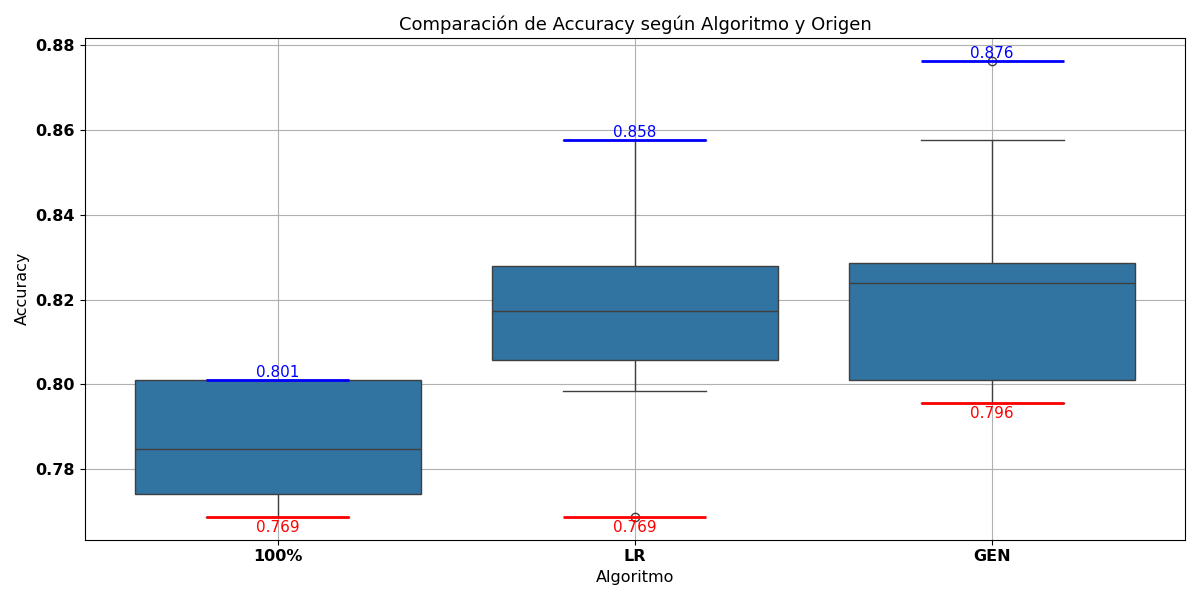
\includegraphics[width=1\textwidth]{imagenes/evaluaciones/comparacion_lr-gen_v1}
    \caption{Boxplot comparando LS con GA usando \textit{accuracy}.}
    \label{fig:lr-vs-gen-v1}
\end{figure}

Tal como se observa en la Figura~\ref{fig:lr-vs-gen-v1}, el algoritmo genético (GA) consigue una \textbf{mediana de \textit{accuracy}} más alta que la búsqueda local (LS),
reflejando un rendimiento medio más consistente.
Además, presenta un valor máximo superior (alcanza hasta \textbf{0.876}), lo que evidencia su mayor potencial para encontrar soluciones de alta calidad.

No obstante, también se aprecia una ligera mayor dispersión en los resultados del GA, particularmente hacia los valores bajos.
Esto indica que, pese a su capacidad exploratoria, el GA puede generar soluciones poco efectivas si no se controlan adecuadamente ciertos operadores como el cruce o la mutación.
De hecho, su valor mínimo (\textbf{0.796}) es superior al de la LS en esta comparativa,
pero deja margen para mejoras en la presión selectiva o en mecanismos que eviten estancamientos.

% \colorbox{yellow}{¿Sobra el siguiente apartado?}
La LS, por su parte, mantiene un comportamiento más estable, aunque con una mediana ligeramente inferior.
Su distribución es más concentrada y limitada en el extremo superior, lo que evidencia su carácter más explotador pero con menor capacidad para alcanzar soluciones óptimas globales.

Estos resultados sirven como evidencia empírica para continuar desarrollando nuevas versiones del GA,
incorporando mejoras específicas en sus operadores con el fin de aprovechar su capacidad exploratoria y, al mismo tiempo, mitigar sus limitaciones.

\section{Mejorando el operador de cruce}\label{sec:incorporacion-cruce}
La primera mejora introducida al GA consiste en reemplazar el cruce aleatorio por un cruce ponderado,
donde se prioriza la contribución del progenitor con mayor \textit{fitness}.
Además, se incorpora una estrategia selectiva que conserva únicamente el mejor de los dos hijos generados en cada cruce.
Ambos cambios, explicados en detalle en la \hyperref[sec:genetico-v2]{Sección~\ref*{sec:genetico-v2}},
buscan aumentar la presión evolutiva y acelerar la convergencia hacia soluciones de mayor calidad,
evitando así que soluciones mediocres se propaguen innecesariamente en la población.

\begin{figure}[htp]
    \centering
    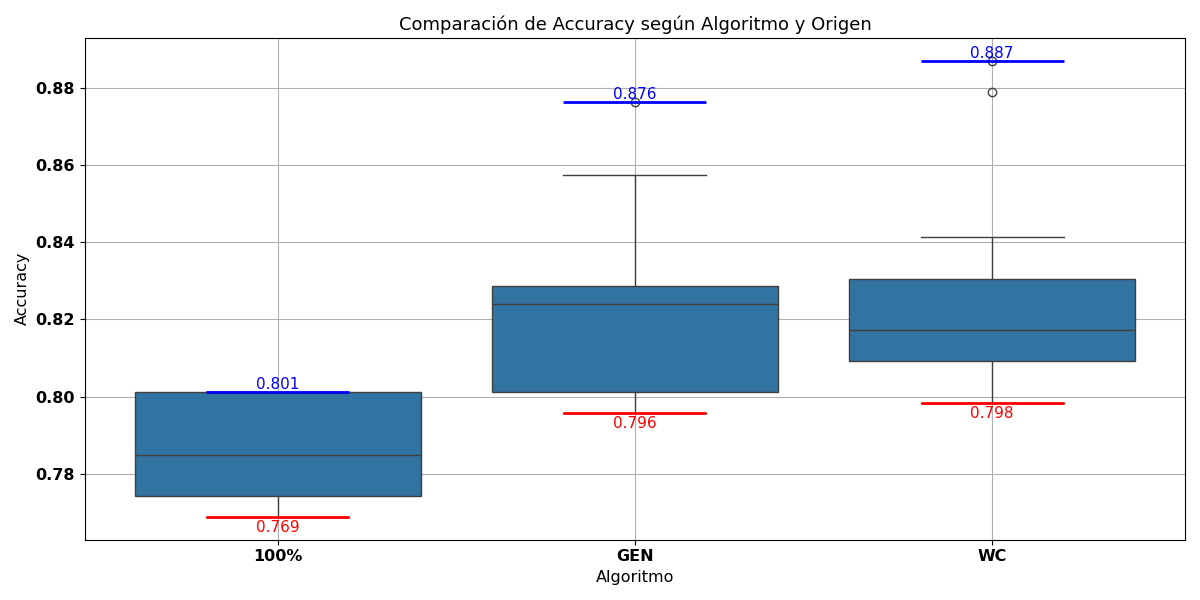
\includegraphics[width=1\textwidth]{imagenes/evaluaciones/operador-de-cruce}
    \caption{Boxplot de \textit{accuracy} comparando el GA y el GA-WC.}
    \label{fig:cruce_ponderado}
\end{figure}

Tal como se observa en la Figura~\ref{fig:cruce_ponderado}, esta modificación produce una mejora clara en la calidad y estabilidad de los resultados.
La versión con cruce ponderado (GA-WC) alcanza un valor máximo atípico superior (\textbf{0.887}),
aunque presenta una mediana más baja que la versión básica (GA).

Pero por otra parte, se aprecia una ligera reducción en la dispersión de los valores inferiores,
con un mínimo de \textbf{0.798} frente al \textbf{0.796} en la versión anterior, lo que sugiere una mayor consistencia.
Aunque el IQR (\hyperref[subsec:visualizacion-de-resultados]{Rango Intercuartílico}) sigue siendo amplio,
la acumulación de valores más cercanos al rango superior refleja una convergencia evolutiva más enfocada y menos dependiente del azar.

En conjunto, esta mejora en el cruce no solo permite una transferencia más eficiente de características ventajosas,
sino que también incrementa la presión selectiva sobre la calidad de las soluciones.
Esto se traduce en un comportamiento más robusto, menos propenso a resultados erráticos y con una mayor capacidad de exploración dirigida del espacio de soluciones.


\section{Mejorando el operador de mutación}\label{sec:mejorando-mutacion}
A partir de los resultados obtenidos con el GA-WC, se evalua una nueva versión en la que se introdujo una \textbf{mutación adaptativa}
(ver \hyperref[sec:genetico-mutacion]{Sección~\ref*{sec:genetico-mutacion}}).
A diferencia de la versión original con tasa fija, esta estrategia ajusta el número de intercambios en función del tamaño del subconjunto mutado,
lo que permite una mayor flexibilidad en escenarios de diferente escala.

\begin{figure}[htp]
    \centering
    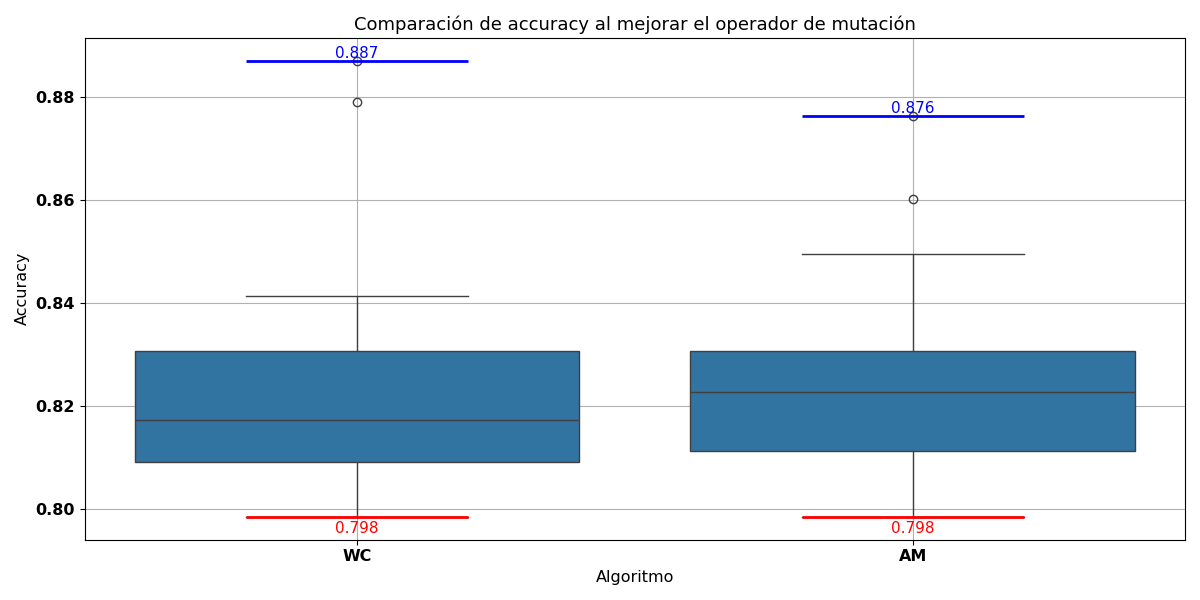
\includegraphics[width=1\textwidth]{imagenes/evaluaciones/mutacion-adaptativa}
    \caption{Comparación de \textit{accuracy} entre el GA-WC y el GA-AM.}
    \label{fig:mutacion-adaptativa}
\end{figure}

\begin{figure}[htp]
    \centering
    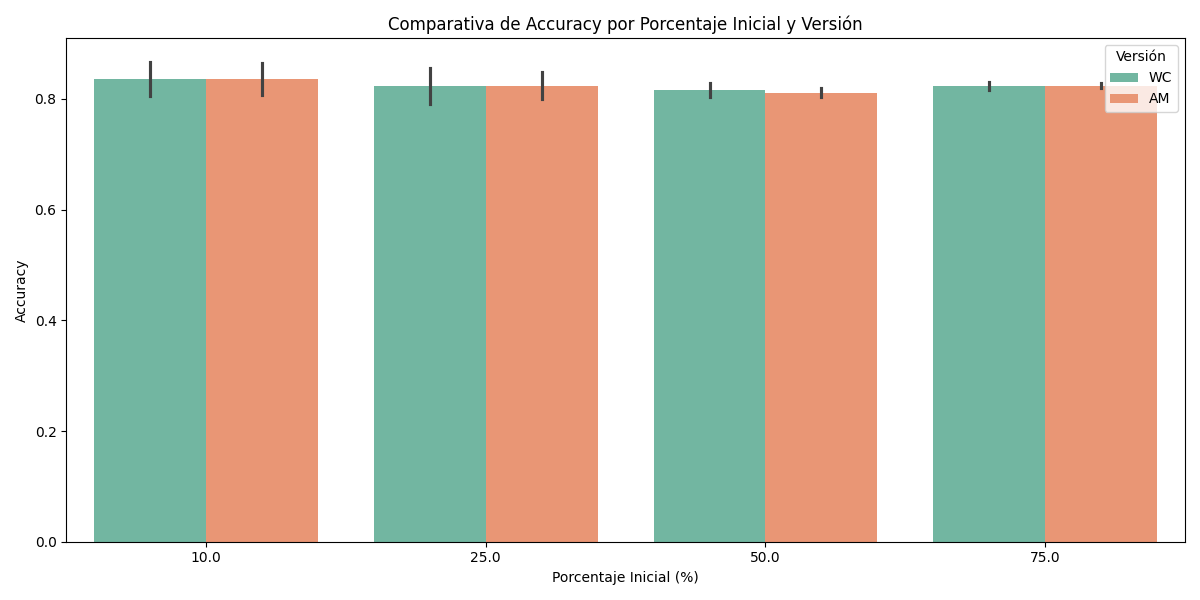
\includegraphics[width=1\textwidth]{imagenes/evaluaciones/mutacion-adaptativa_por_porcentaje}
    \caption{Diagrama de comparación usando el \textit{accuracy} entre el GA-WC Y el GA-AM, separados por porcentaje inicial.}
    \label{fig:mutacion-adaptativa-porcentaje}
\end{figure}

Como se aprecia en la Figura~\ref{fig:mutacion-adaptativa},
ambos algoritmos presentan distribuciones de \textit{accuracy} muy similares en términos de mediana e IQR.
El GA-WC mantiene un ligero máximo superior, alcanzando un \textbf{0.887} frente al \textbf{0.876} del GA-AM.
Sin embargo, el algoritmo con mutación adaptativa muestra una distribución más compacta en la parte central,
con menor dispersión hacia valores bajos, lo que sugiere una mayor consistencia entre ejecuciones.

La principal diferencia se observa en la robustez de los resultados: el GA-AM presenta una distribución más estable,
con menos valores atípicos y una mayor concentración de ejecuciones cerca del cuartil superior.
Este comportamiento indica una menor propensión a caídas abruptas de rendimiento y refuerza la idea de que la mutación
adaptativa mejora la estabilidad del proceso evolutivo.

Al analizar los resultados por porcentaje inicial (Figura~\ref{fig:mutacion-adaptativa-porcentaje}),
se confirma que el GA-AM mantiene una estabilidad más uniforme en todos los escenarios, mientras que el GA-WC muestra una mayor variabilidad,
especialmente en configuraciones con menor cantidad de datos.
Aunque las diferencias en \textit{accuracy} medio no son significativas, la menor dispersión y la reducción de valores extremos justifican la
preferencia por la versión adaptativa en contextos donde la fiabilidad es prioritaria.

En conjunto, la mutación adaptativa no genera una mejora radical en precisión media,
pero sí contribuye a una evolución más controlada y menos susceptible a degradaciones, favoreciendo una mayor consistencia en los resultados.
Además, al adaptarse al tamaño del subconjunto, evita configuraciones subóptimas que podrían surgir con una tasa fija de mutación,
lo que la hace especialmente adecuada para escenarios con escalas variables.

Esta mejora consolida la capacidad del algoritmo para equilibrar exploración y explotación,
y lo posiciona como una alternativa más robusta y estable en tareas de reducción de datos para aprendizaje profundo.


\section{Resultados del reinicio poblacional}\label{sec:resultados-reinicio-poblacional}
La última mejora realizada de los algoritmos genéticos (ver \hyperref[sec:genetico-v3]{Sección~\ref*{sec:genetico-v3}})
introduce una lógica de reinicio poblacional diseñada para evitar estancamientos evolutivos.
El algoritmo monitoriza el rendimiento del segundo mejor individuo, y si este no mejora durante dos generaciones consecutivas,
se aplica un reinicio parcial que conserva únicamente al mejor individuo de la población.

\begin{figure}[htp]
    \centering
    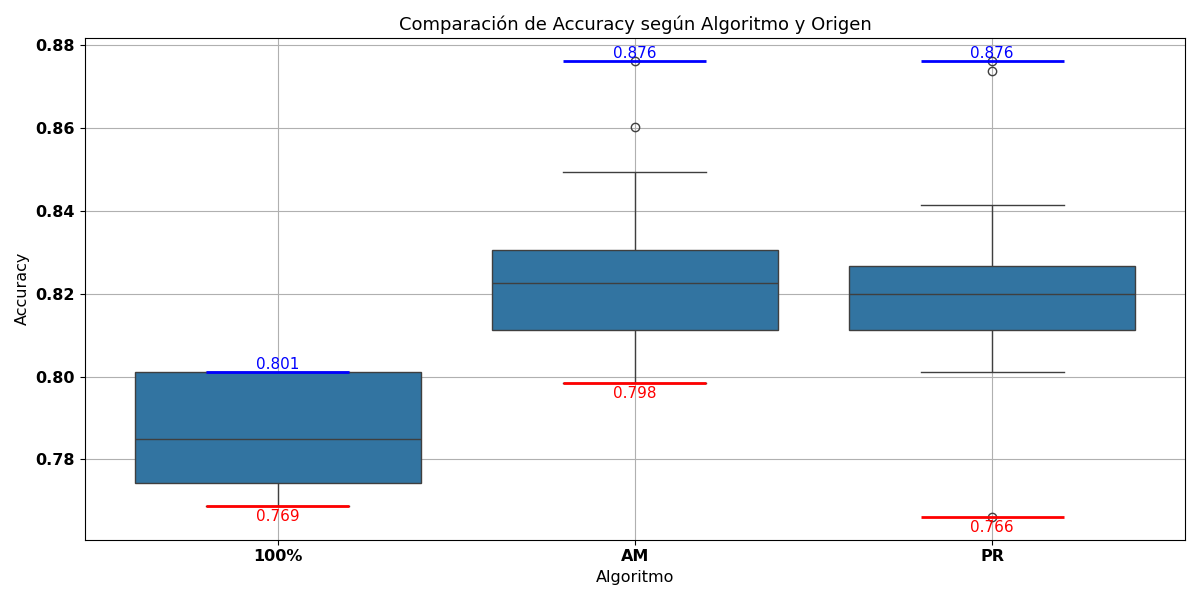
\includegraphics[width=1\textwidth]{imagenes/evaluaciones/reinicio-poblacional}
    \caption{Comparación de \textit{accuracy} entre el GA-AM y con PR.}
    \label{fig:reinicio_poblacional}
\end{figure}
\begin{table}[htp]
    \centering
    \resizebox{\textwidth}{!}{
        \begin{tabular}{P{2cm} P{2cm} P{2.5cm} P{2.5cm} P{2.5cm} P{2.5cm} P{2cm} P{2cm} P{2cm} P{2cm} P{2cm} P{2.5cm} P{2.5cm}}
            \toprule
            \textbf{Algoritmo}    & \textbf{Duración Total} & \textbf{Duración por Eval.} & \textbf{Accuracy (Avg)} & \textbf{Precision (Avg)} &
            \textbf{Recall (Avg)} & \textbf{F1-score (Avg)} & \textbf{Evaluaciones}       & \textbf{Porc.Paper}     & \textbf{Porc.Rock}       & \textbf{Porc.Scissors}                                               \\
            \midrule
            \multicolumn{11}{l}{\textbf{10\%}}                                                                                                                                                                        \\
            \midrule
            GA-AM                 & 00:27:39                & 00:00:17                    & 83,66\%                 & 84,24\%                  & 83,66\%                & 83,09\% & 100 & 35,64\% & 30,87\% & 33,49\% \\
            PR                    & 00:29:02                & 00:00:17                    & 81,93\%                 & 83,07\%                  & 81,93\%                & 81,19\% & 100 & 34,52\% & 32,14\% & 33,33\% \\
            \midrule
            \multicolumn{11}{l}{\textbf{25\%}}                                                                                                                                                                        \\
            \midrule
            GA-AM                 & 00:57:29                & 00:00:34                    & 82,42\%                 & 83,68\%                  & 82,42\%                & 81,78\% & 100 & 33,33\% & 32,54\% & 34,13\% \\
            PR                    & 01:00:22                & 00:00:36                    & 82,64\%                 & 83,78\%                  & 82,64\%                & 81,96\% & 100 & 33,62\% & 33,27\% & 33,11\% \\
            \midrule
            \multicolumn{11}{l}{\textbf{50\%}}                                                                                                                                                                        \\
            \midrule
            GA-AM                 & 01:47:31                & 00:01:05                    & 81,13\%                 & 82,62\%                  & 81,13\%                & 80,41\% & 100 & 33,94\% & 32,76\% & 33,30\% \\
            PR                    & 01:53:13                & 00:01:08                    & 81,24\%                 & 83,09\%                  & 81,24\%                & 80,59\% & 100 & 33,21\% & 33,20\% & 33,59\% \\
            \midrule
            \multicolumn{11}{l}{\textbf{75\%}}                                                                                                                                                                        \\
            \midrule
            GA-AM                 & 02:36:41                & 00:01:34                    & 82,42\%                 & 83,94\%                  & 82,42\%                & 81,85\% & 100 & 33,67\% & 33,11\% & 33,22\% \\
            PR                    & 02:41:24                & 00:01:37                    & 82,69\%                 & 84,33\%                  & 82,69\%                & 82,06\% & 100 & 33,52\% & 33,44\% & 33,04\% \\
            \midrule
            \multicolumn{11}{l}{\textbf{100\%}}                                                                                                                                                                       \\
            \midrule
            100\%                 & -                       & 00:03:16                    & 78,60\%                 & 81,55\%                  & 78,60\%                & 77,68\% & 1   & 33,33\% & 33,33\% & 33,33\% \\
            \bottomrule
        \end{tabular}
    }
    \caption{Resultados de los algoritmos GA-AM y PR por porcentaje inicial, incluyendo distribución de clases y duración total y por evaluación.}
    \label{tab:resultados-am-pr-porcentaje}
\end{table}

Los resultados, mostrados en la Figura~\ref{fig:reinicio_poblacional} y la Tabla~\ref{tab:resultados-am-pr-porcentaje},
permiten extraer varias conclusiones relevantes.
En primer lugar, el \textbf{valor máximo de accuracy} es idéntico para GA-AM y PR, alcanzando ambos un \textbf{0.876},
lo que sugiere que el reinicio no favorece la aparición de soluciones de mayor calidad.
Por el contrario, el \textbf{valor mínimo de accuracy} observado en PR (\textbf{0.766}) es notablemente más bajo que el de GA-AM (\textbf{0.798}),
lo que indica una mayor propensión a obtener ejecuciones de bajo rendimiento cuando se utiliza la estrategia de reinicio.

La distribución general de resultados revela que el PR no logra una reducción significativa en la dispersión de los valores:
aunque los cuartiles y medianas de GA-AM y PR son similares, se observa un leve desplazamiento hacia valores ligeramente más bajos en PR,
lo cual es especialmente evidente en el escenario de menor porcentaje inicial (10\%).
Esta tendencia sugiere que el reinicio poblacional, al reintroducir diversidad de forma abrupta,
puede generar soluciones subóptimas que no contribuyen de manera sustancial a mejorar la población.

La tabla de resultados~\ref{tab:resultados-am-pr-porcentaje} respalda estas observaciones: en promedio,
el algoritmo GA-AM presenta una ligera superioridad en precisión media (\textbf{83,66\%} frente a \textbf{81,93\%} en el 10\%), así como en F1-score y recall.
Estas diferencias, aunque no drásticas, son consistentes en la mayoría de los escenarios.
Además, las métricas de distribución de clases y las duraciones de ejecución son prácticamente equivalentes entre GA-AM y PR,
lo que refuerza la idea de que el impacto del reinicio poblacional no justifica su complejidad añadida.

% \colorbox{yellow}{¿Añadir el párrafo de resumen?}
% En resumen, aunque el reinicio poblacional es una estrategia teóricamente útil para escapar de óptimos locales,
% su implementación en esta versión no logró aportar beneficios consistentes en términos de rendimiento.
% Estos resultados invitan a reconsiderar su activación por defecto, o bien a explorar variantes más refinadas del mecanismo de reinicio.
En resumen, aunque el reinicio poblacional busca aumentar la exploración y evitar el estancamiento,
en esta implementación concreta no aporta mejoras tangibles en términos de precisión ni estabilidad,
e incluso puede introducir soluciones más erráticas en ciertas ejecuciones.

\section{Resultados con versiones libres}\label{sec:resultados-versiones-libres}
Como parte de la evolución de los algoritmos desarrollados, se propone la creación de \textbf{versiones libres},
en las que el tamaño del subconjunto seleccionado no permanece fijo durante la ejecución, sino que puede ajustarse de forma dinámica en función de las decisiones evolutivas.
Esta flexibilidad permite que los algoritmos modifiquen el número de datos utilizados a medida que avanzan las generaciones,
adaptándose de manera más natural a las características del problema.

Para evaluar el impacto de esta modificación, se generan versiones libres tanto para el algoritmo de búsqueda local (LS)
como para el algoritmo con mutación adaptativa (GA-AM).
En el caso de la LS, además, se incorpora una variación adicional: el porcentaje inicial de imágenes no es fijo,
sino que se selecciona aleatoriamente en cada ejecución, introduciendo así un mayor grado de aleatoriedad y diversidad en el proceso.


\begin{figure}[htp]
    \centering
    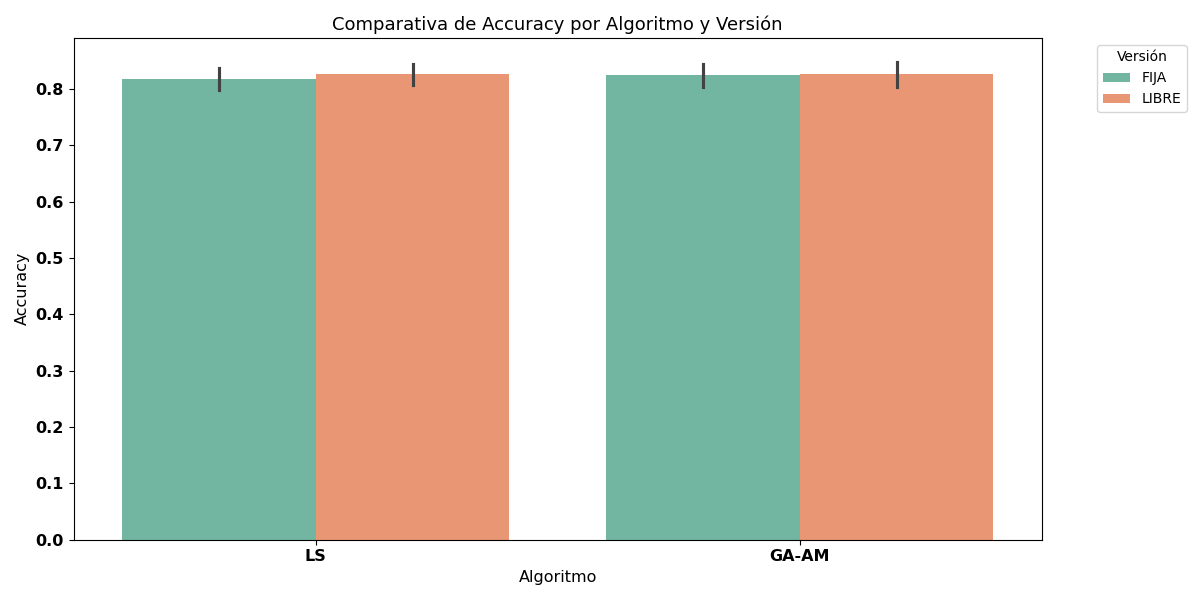
\includegraphics[width=0.9\textwidth]{imagenes/evaluaciones/libres/barplot_por_algoritmo}
    \caption{Comparación de \textit{accuracy} entre el LS, GA-AM y sus versiones Libres (formato BARPLOT).}
    \label{fig:barplot_por_algoritmo-libres}
\end{figure}

En la Figura~\ref{fig:barplot_por_algoritmo-libres} se observa que las versiones libres mantienen un rendimiento promedio muy similar al de las versiones originales.
La precisión media (\textit{accuracy}) de las versiones libres es ligeramente superior en algunos casos,
lo que indica que la capacidad de adaptación no introduce pérdidas de rendimiento e incluso puede aportar pequeñas mejoras en escenarios específicos.
Las barras de error sugieren que la variabilidad entre ejecuciones se mantiene controlada,
lo que refuerza la idea de que la flexibilidad no compromete la estabilidad de los resultados.


\begin{figure}[htp]
    \centering
    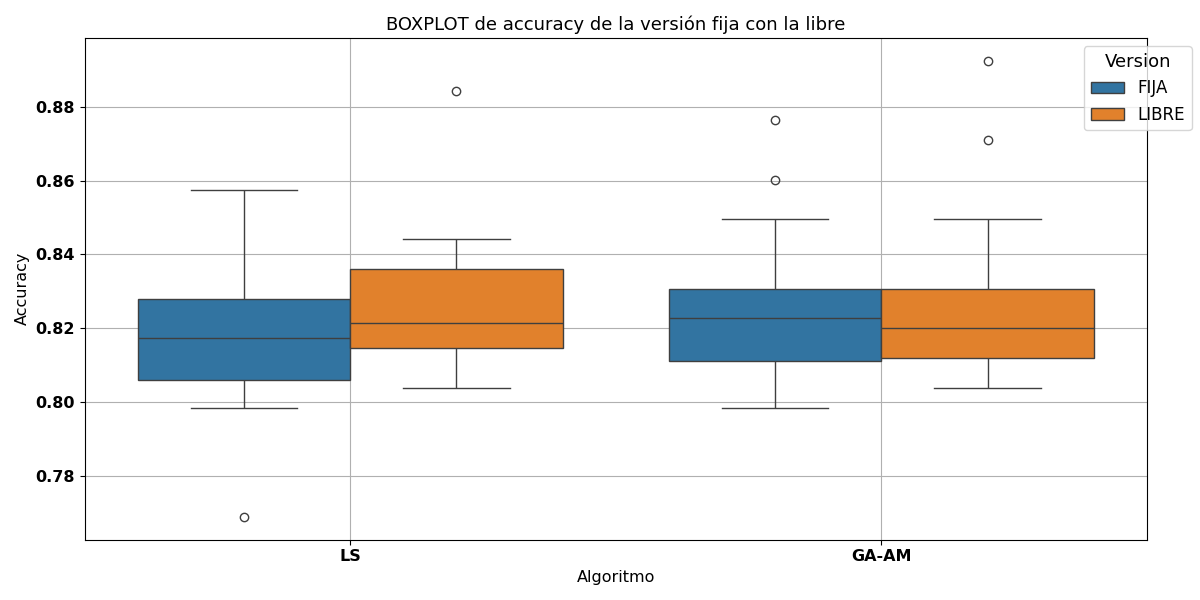
\includegraphics[width=0.9\textwidth]{imagenes/evaluaciones/libres/boxplot_por_algoritmo}
    \caption{Comparación de \textit{accuracy} entre el LS, GA-AM y sus versiones Libres en formato BOXPLOT.}
    \label{fig:boxplot_por_algoritmo-libres}
\end{figure}

Los diagramas de caja en la Figura~\ref{fig:boxplot_por_algoritmo-libres} permiten una comparación más detallada de la dispersión de los resultados.
En el caso de la LS, la versión libre muestra una ligera mejora en la mediana y un rango intercuartílico (IQR) más compacto, lo que indica una mayor estabilidad.
Además, se observan valores atípicos superiores que sugieren la posibilidad de obtener ejecuciones con precisión especialmente alta.
En el caso del GA-AM, las diferencias entre las versiones fija y libre son más sutiles: aunque las medianas son prácticamente idénticas,
la versión libre presenta una ligera reducción en los valores mínimos, lo que podría reflejar una mayor adaptabilidad frente a escenarios más difíciles.


\begin{figure}[htp]
    \centering
    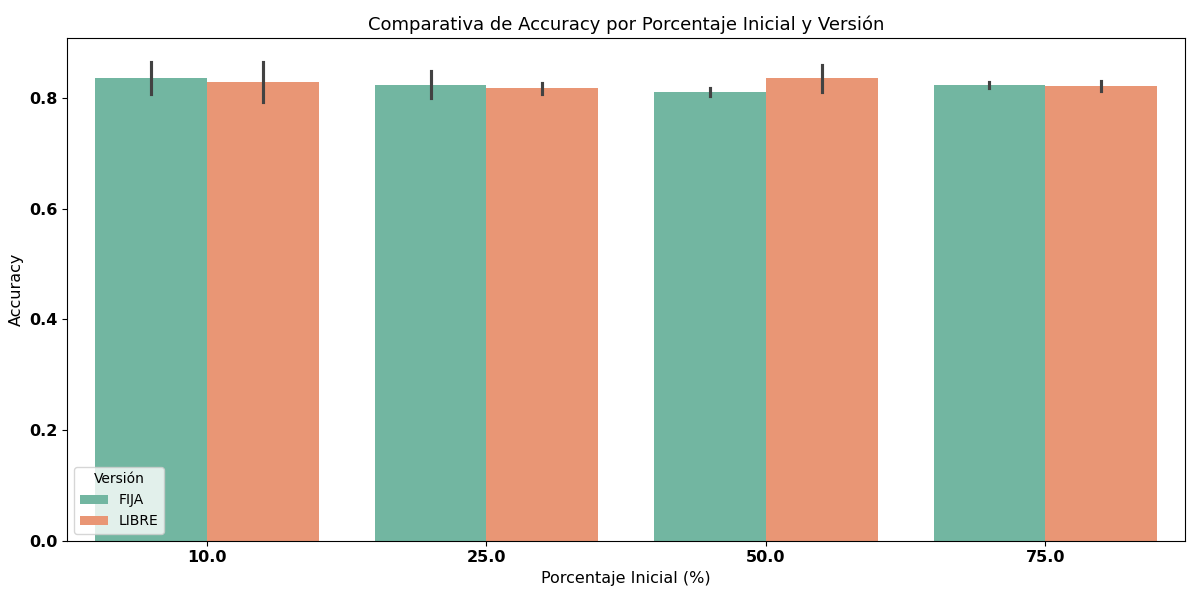
\includegraphics[width=0.9\textwidth]{imagenes/evaluaciones/libres/am_por_pi}
    \caption{Comparación de \textit{accuracy} en función del porcentaje inicial para el algoritmo GA-AM.}
    \label{fig:am_por_pi}
\end{figure}

La Figura~\ref{fig:am_por_pi} muestra la evolución del \textit{accuracy} en función del porcentaje inicial de datos utilizados en el algoritmo GA-AM.
Se observa que la precisión se mantiene estable a lo largo de los distintos puntos de partida,
con ligeras variaciones que no afectan de manera significativa al comportamiento general del algoritmo.
Este resultado confirma que la flexibilidad en el tamaño del subconjunto no introduce un sesgo negativo en la calidad de las soluciones encontradas,
sino que permite adaptarse a diferentes condiciones iniciales sin comprometer el rendimiento.


\begin{figure}[htp]
    \centering
    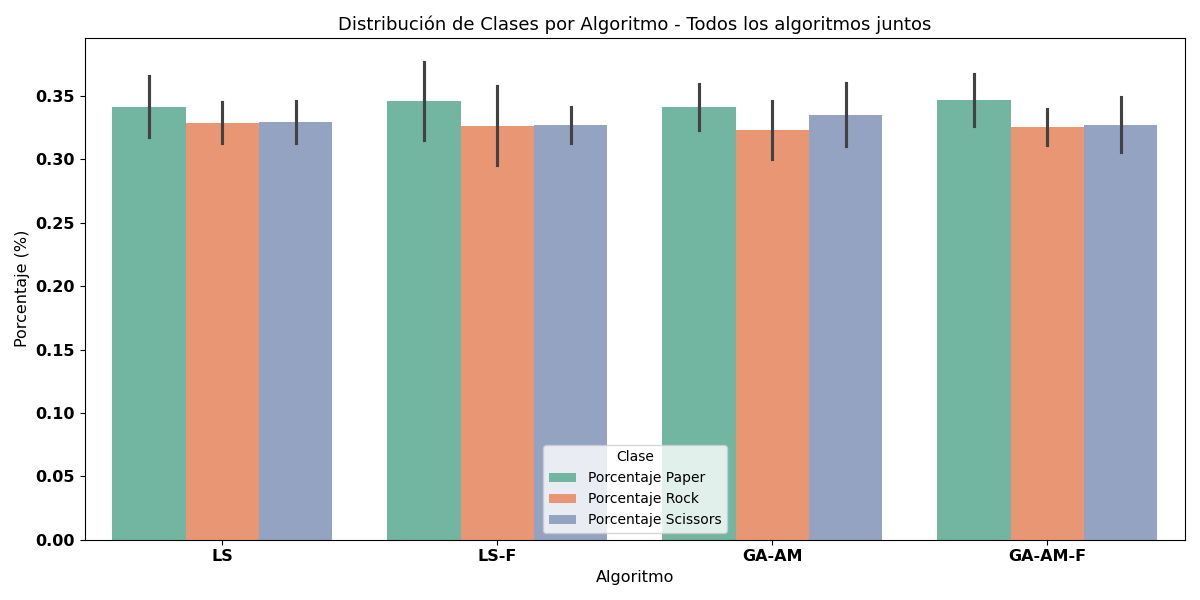
\includegraphics[width=0.9\textwidth]{imagenes/evaluaciones/libres/distribucion-clases}
    \caption{Distribución de clases en los subconjuntos generados por los algoritmos estándar y libres.}
    \label{fig:distribucion_libres}
\end{figure}

Por otro lado, la Figura~\ref{fig:distribucion_libres} demuestra que tanto las versiones fijas como las libres preservan una
distribución equilibrada de las clases \texttt{Rock}, \texttt{Paper} y \texttt{Scissors}.
Las proporciones entre clases se mantienen estables, sin que la flexibilidad en el tamaño del subconjunto genere desbalances significativos.
Este aspecto es crucial, ya que garantiza la validez de los experimentos y asegura que las mejoras observadas no son producto de un sesgo de clase inadvertido.


\begin{figure}[htp]
    \centering
    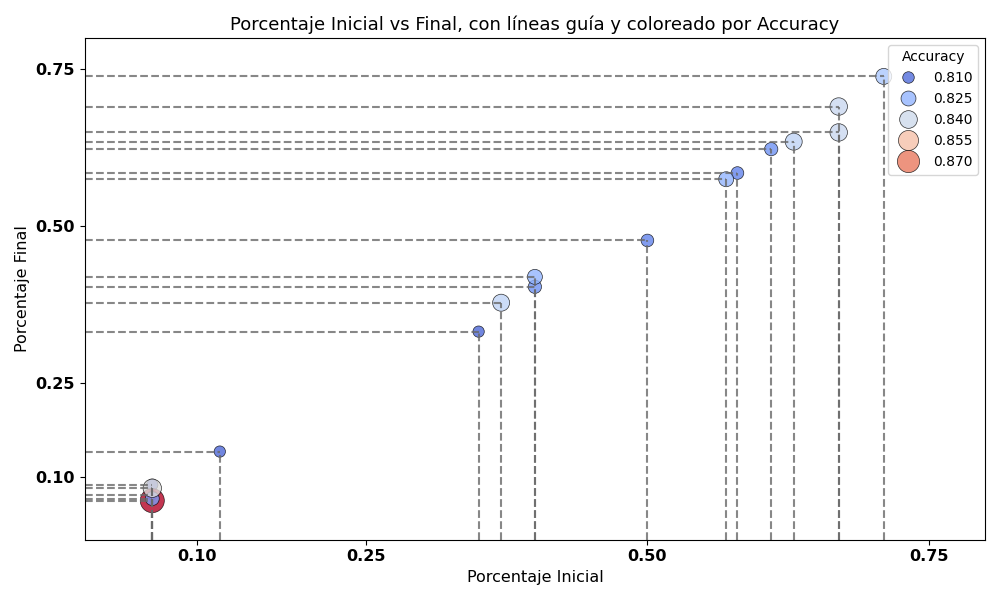
\includegraphics[width=0.9\textwidth]{imagenes/evaluaciones/libres/scatter_lr-f}
    \caption{Relación entre \textit{accuracy} y porcentaje final de datos seleccionados por el algoritmo LS-F.}
    \label{fig:scatter_bl_f}
\end{figure}

\begin{figure}[htp]
    \centering
    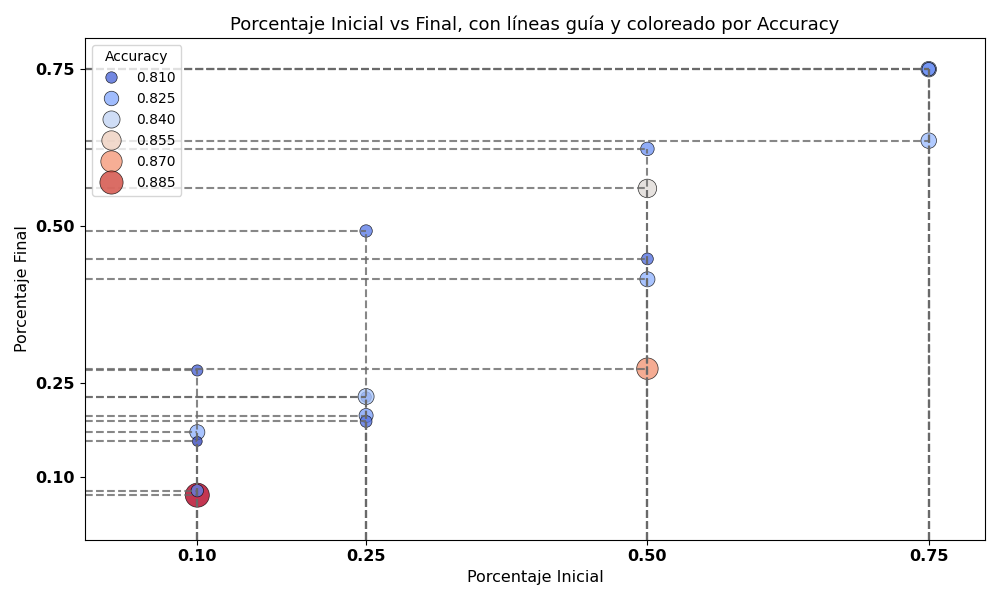
\includegraphics[width=0.9\textwidth]{imagenes/evaluaciones/libres/scatter_gen_v2}
    \caption{Relación entre \textit{accuracy} y porcentaje final de datos seleccionados por el algoritmo GA-AM-F.}
    \label{fig:scatter_gen_v2}
\end{figure}

Finalmente, las Figuras~\ref{fig:scatter_bl_f} y~\ref{fig:scatter_gen_v2} permiten visualizar la relación entre el \textit{accuracy}
y el porcentaje final de datos seleccionados en las versiones libres.
En el caso de la búsqueda local libre (LS-F), se observa una tendencia a incrementar ligeramente el tamaño del subconjunto final,
especialmente en ejecuciones con mejor precisión.
Por el contrario, el algoritmo GA-AM-F muestra una distribución más equilibrada, con una mayor variabilidad en los tamaños finales,
lo que refleja su capacidad adaptativa para ajustarse a diferentes condiciones de búsqueda.

Este comportamiento evidencia que los algoritmos libres no solo adaptan la composición del subconjunto, sino también su escala,
ajustando dinámicamente la cantidad de datos utilizados según las necesidades del proceso evolutivo.
En conjunto, estas versiones demuestran ser una alternativa más versátil y robusta,
capaz de mantener la calidad del rendimiento incluso en escenarios con alta variabilidad en los datos o restricciones de tamaño no conocidas de antemano.


\section{Resultados del algoritmo memético}\label{sec:resultados-algoritmo-memetico}
Finalmente, se evalua el algoritmo memético (MA) (ver \hyperref[sec:algoritmo-memetico]{Sección~\ref*{sec:algoritmo-memetico}}),
el cual combina la evolución genética con una búsqueda local aplicada de forma probabilística sobre ciertos individuos seleccionados.
Este enfoque híbrido busca equilibrar la exploración del espacio de soluciones con una intensificación localizada,
ofreciendo mejoras tanto en precisión como en estabilidad.


\begin{figure}[htp]
    \centering
    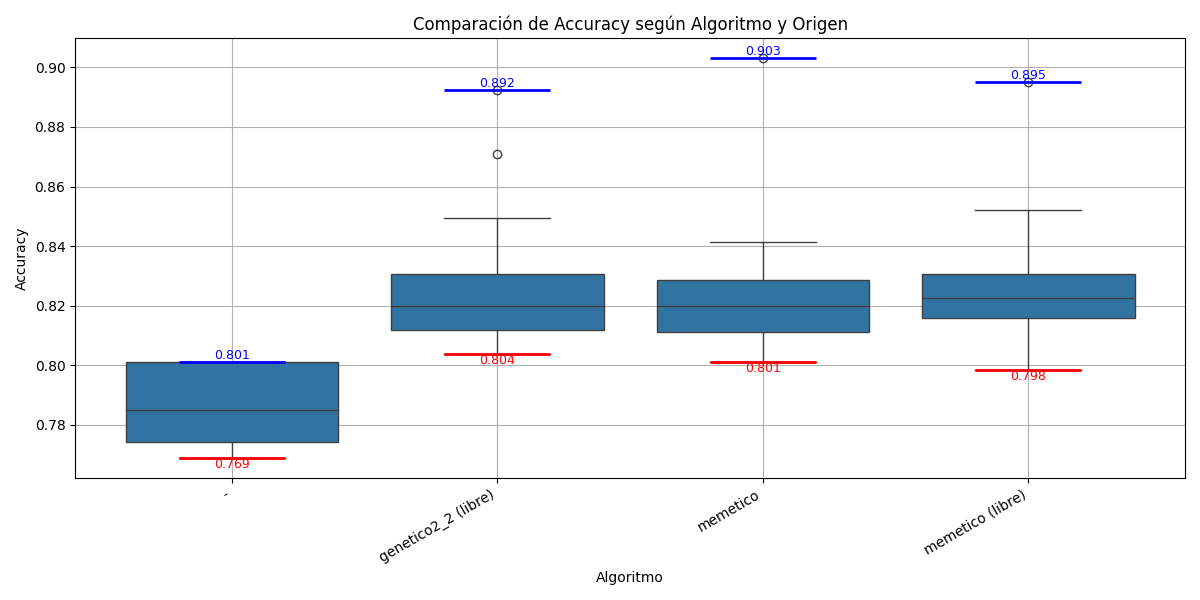
\includegraphics[width=0.9\textwidth]{imagenes/evaluaciones/comparacion-memetico}
    \caption{Comparación de \textit{accuracy} entre el algoritmo memético (MA) y su versión libre.}
    \label{fig:memetico_comparacion}
\end{figure}

Tal como se aprecia en la Figura~\ref{fig:memetico_comparacion}, el algoritmo memético (MA) supera claramente al mejor de los enfoques genéticos
(GA-AM-F), alcanzando una mediana más elevada y un valor máximo de \textit{accuracy} de hasta \textbf{0.903}.
Su distribución es más compacta, con menor dispersión hacia los valores bajos, lo que refleja una mayor consistencia entre ejecuciones.

La versión libre del memético, que incorpora también un ajuste dinámico del tamaño del subconjunto
(ver \hyperref[subsec:memetico-libre]{Apartado~\ref*{subsec:memetico-libre}}), muestra un rendimiento muy similar al estándar,
con una ligera reducción en el valor máximo pero una estabilidad comparable.
Esto sugiere que el componente adaptativo no penaliza la calidad de las soluciones y puede incluso aportar mayor flexibilidad en entornos más inciertos.


\begin{table}[htp]
    \centering
    \resizebox{\textwidth}{!}{
        \begin{tabular}{P{2.2cm} P{2.2cm} P{2.2cm} P{2.2cm} P{2.2cm} P{2.2cm} P{2cm} P{2.5cm} P{2.5cm}}
            \toprule
            \textbf{Algoritmo}    & \textbf{Duración Total} & \textbf{Duración por Eval.} & \textbf{Porc.
            Final}                & \textbf{Accuracy (Avg)} & \textbf{Precision (Avg)}    &
            \textbf{Recall (Avg)} & \textbf{F1-score (Avg)} & \textbf{Evaluaciones}                                                                     \\
            \midrule
            \multicolumn{9}{l}{\textbf{10\%}}                                                                                                           \\
            \midrule
            GA-AM-F               & 00:34:33                & 00:00:21                    & 14,94\%       & 82,96\% & 84,07\% & 82,96\% & 82,12\% & 100 \\
            MA                    & 00:27:43                & 00:00:17                    & 10,00\%       & 82,85\% & 84,44\% & 82,85\% & 81,91\% & 100 \\
            MA-F                  & 00:32:39                & 00:00:20                    & 9,62\%        & 83,28\% & 84,70\% & 83,28\% & 82,46\% & 100 \\
            \midrule
            \multicolumn{9}{l}{\textbf{25\%}}                                                                                                           \\
            \midrule
            GA-AM-F               & 01:07:13                & 00:00:40                    & 26,68\%       & 81,77\% & 82,66\% & 81,77\% & 81,18\% & 100 \\
            MA                    & 00:57:12                & 00:00:34                    & 25,00\%       & 81,99\% & 83,11\% & 81,99\% & 81,21\% & 100 \\
            MA-F                  & 01:08:54                & 00:00:41                    & 27,18\%       & 82,80\% & 83,77\% & 82,80\% & 82,17\% & 100 \\
            \midrule
            \multicolumn{9}{l}{\textbf{50\%}}                                                                                                           \\
            \midrule
            GA-AM-F               & 01:51:24                & 00:01:07                    & 46,36\%       & 83,60\% & 85,22\% & 83,60\% & 83,03\% & 100 \\
            MA                    & 01:47:32                & 00:01:05                    & 50,00\%       & 81,51\% & 83,36\% & 81,51\% & 80,89\% & 100 \\
            MA-F                  & 02:16:51                & 00:01:22                    & 67,07\%       & 81,61\% & 83,09\% & 81,61\% & 80,96\% & 100 \\
            \midrule
            \multicolumn{9}{l}{\textbf{75\%}}                                                                                                           \\
            \midrule
            GA-AM-F               & 02:33:25                & 00:01:32                    & 72,72\%       & 82,20\% & 83,94\% & 82,20\% & 81,47\% & 100 \\
            MA                    & 02:37:43                & 00:01:35                    & 75,00\%       & 82,74\% & 84,33\% & 82,74\% & 82,14\% & 100 \\
            MA-F                  & 03:08:21                & 00:01:53                    & 71,16\%       & 82,69\% & 84,18\% & 82,69\% & 82,10\% & 100 \\
            \midrule
            \multicolumn{9}{l}{\textbf{100\%}}                                                                                                          \\
            \midrule
            100\%                 & -                       & 00:03:16                    & 100,00\%      & 78,60\% & 81,55\% & 78,60\% & 77,68\% & 1   \\
            \bottomrule
        \end{tabular}
    }
    \caption{Resultados de los MA y del GA-AM-F por porcentaje inicial.}
    \label{tab:resultados-memetico-genetico-libres}
\end{table}

El análisis detallado de la Tabla~\ref{tab:resultados-memetico-genetico-libres} confirma estas observaciones y permite extraer
conclusiones más matizadas sobre el comportamiento de los algoritmos.
En primer lugar, el MA-F mantiene una precisión media comparable o superior a la del MA en la mayoría de los escenarios,
especialmente en configuraciones con porcentajes iniciales más bajos (10\% y 25\%).
Esto indica que la capacidad de ajuste dinámico no solo no perjudica el rendimiento, sino que puede ofrecer ventajas en términos de adaptabilidad,
permitiendo al algoritmo optimizar la selección de datos sin depender de un tamaño fijo preestablecido.

Además, el porcentaje final alcanzado por MA-F muestra una notable variabilidad según el escenario:
en los casos con menor porcentaje inicial, tiende a mantenerse cercano al valor de partida (por ejemplo, un 9,62\% en el escenario del 10\%),
mientras que en configuraciones más amplias (50\% y 75\%), el tamaño final puede incrementarse significativamente (hasta un 67,07\% en el caso del 50\%).
Este comportamiento adaptativo refleja que el algoritmo es capaz de ajustar la escala de la solución en función de las características del espacio de búsqueda,
evitando tanto la sobrerrepresentación como la selección excesiva de datos innecesarios.

Por otro lado, la duración total y el tiempo medio por evaluación aumentan con el porcentaje inicial, pero esto no compromete la eficiencia general del MA-F,
que mantiene un equilibrio adecuado entre precisión y coste computacional

De esta forma, tanto el MA como su variante libre, MA-F, se consolidan como las estrategias más eficaces del estudio,
ofreciendo una combinación robusta de rendimiento, adaptabilidad y estabilidad.

% \colorbox{yellow}{¿Añadir el párrafo de resumen?}
% Su combinación de precisión elevada, estabilidad entre ejecuciones y capacidad adaptativa los convierte en soluciones
% especialmente robustas para tareas donde se requiere seleccionar subconjuntos representativos sin comprometer el rendimiento del modelo entrenado.

\section{Resultados finales entre enfoques}\label{sec:comparacion-final-enfoques}
Tras analizar el rendimiento individual de cada enfoque a lo largo de las secciones anteriores,
en esta sección se realiza una síntesis comparativa entre los principales algoritmos desarrollados: el algoritmo genético con cruce ponderado (\texttt{GA-WC}), el algoritmo genético con mutación adaptativa (\texttt{GA-AM}), el algoritmo memético (\texttt{MA}) y su versión libre (\texttt{MA-F}).
Se incluyen además las referencias al 100\% del conjunto de datos y a la selección aleatoria (\texttt{RS})
como líneas base para contextualizar los resultados.

El objetivo es identificar cuál de estos enfoques logra el mejor compromiso entre precisión (\textit{accuracy}),
estabilidad de resultados, y eficiencia en la reducción de datos, así como validar la hipótesis de que una selección inteligente de ejemplos puede superar incluso al uso del 100\% del conjunto de datos.

\subsection{Análisis comparativo de accuracy}\label{sec:comparacion-final-accuracy}
\begin{figure}[htp]
    \centering
    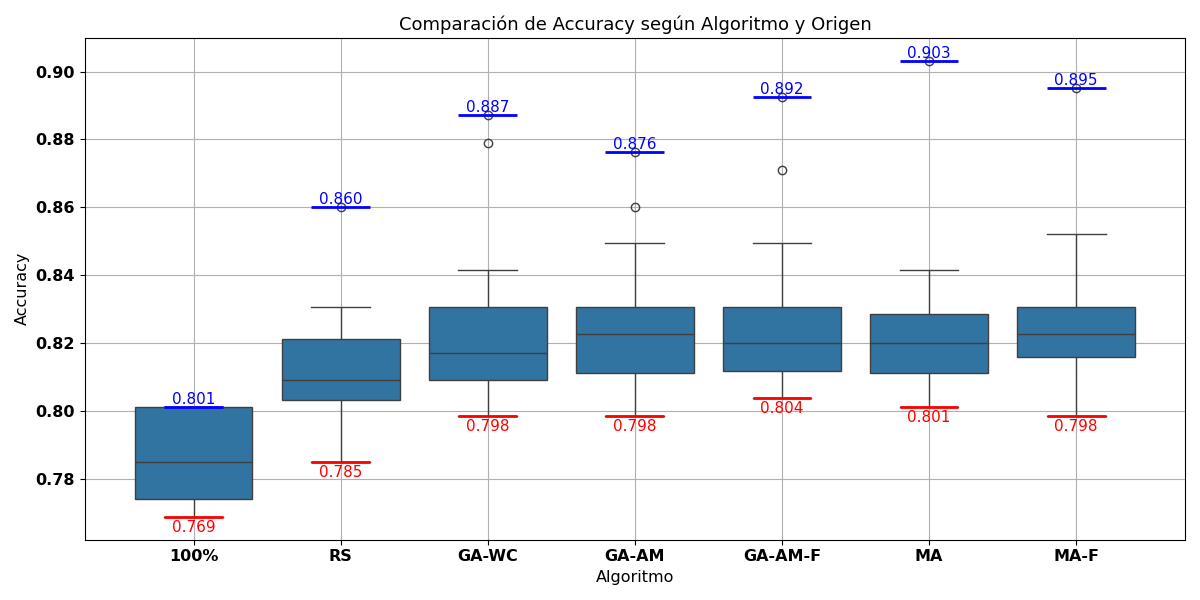
\includegraphics[width=0.95\textwidth]{imagenes/evaluaciones/final/boxplot-por-algoritmo}
    \caption{Boxplot de \textit{accuracy} para los algoritmos RS, GA-WC, GA-AM, MA y MA-F.}
    \label{fig:boxplot-comparacion-final}
\end{figure}
El análisis comparativo de \textit{accuracy} entre algoritmos confirma de manera general las conclusiones obtenidas en los análisis de las secciones anteriores.
Como muestra el boxplot~\ref{fig:boxplot-comparacion-final}, los algoritmos meméticos, especialmente la versión libre \texttt{MA-F},
presentan las mejores métricas globales en términos de precisión y estabilidad.
\texttt{MA-F} alcanza las medianas más altas y muestra una distribución más compacta, lo que refleja una mayor consistencia entre ejecuciones.
Además, la dispersión de resultados en \texttt{MA-F} es menor, lo que sugiere una robustez notable frente a la aleatoriedad de las ejecuciones y una mayor fiabilidad en su rendimiento.

Por otro lado, el algoritmo memético estándar \texttt{MA} también destaca por su rendimiento superior,
aunque presenta una ligera mayor variabilidad en algunos casos.
Aun así, se posiciona como una solución altamente efectiva,
confirmando que la combinación de evolución global y búsqueda local permite generar subconjuntos más representativos y eficientes.

En contraste, los algoritmos \texttt{RS} y \texttt{GA-WC} muestran una mayor dispersión en los resultados,
lo que indica una menor estabilidad y una mayor dependencia de la aleatoriedad en la selección de datos.
\texttt{RS}, como se ha observado a lo largo de todo el análisis, tiende a obtener resultados más erráticos, mientras que \texttt{GA-WC},
aunque introduce mejoras respecto al \texttt{RS}, sigue sin alcanzar la solidez de los algoritmos meméticos.

Por su parte, el algoritmo \texttt{GA-AM} presenta un rendimiento intermedio: mejora las métricas obtenidas por \texttt{RS} y \texttt{GA-WC},
pero no logra superar la precisión ni la estabilidad de los algoritmos meméticos.
Esto refuerza la hipótesis planteada a lo largo del análisis de los resultados: los enfoques basados en algoritmos meméticos,
especialmente en su versión libre, permiten alcanzar una combinación óptima de precisión,
reducción de datos y estabilidad en problemas de selección de instancias para modelos de aprendizaje profundo.

\subsection{Porcentaje final de datos seleccionados}\label{sec:porcentaje-final-datos-seleccionados}
\begin{figure}[htp]
    \centering
    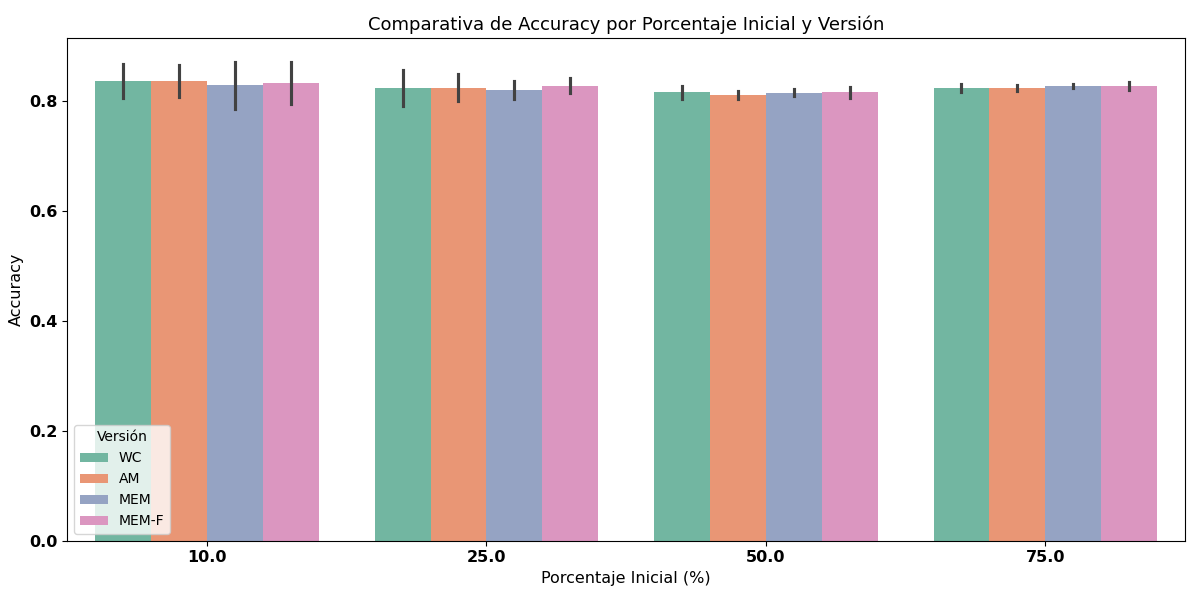
\includegraphics[width=0.95\textwidth]{imagenes/evaluaciones/final/barplot-por-porcentaje}
    \caption{Porcentaje final de datos seleccionados por cada algoritmo.}
    \label{fig:barplot-por-porcentaje}
\end{figure}
\begin{figure}[htp]
    \centering
    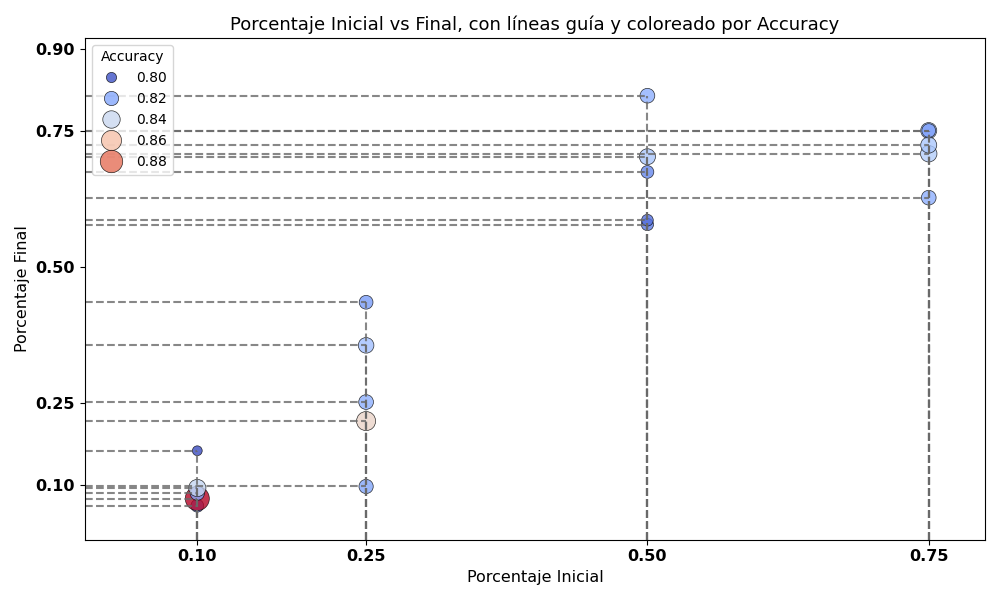
\includegraphics[width=0.95\textwidth]{imagenes/evaluaciones/final/scatter}
    \caption{Relación entre \textit{accuracy} y porcentaje final de datos seleccionados por cada algoritmo.}
    \label{fig:scatter-final}
\end{figure}El análisis del porcentaje final de datos seleccionados permite evaluar la eficiencia de cada algoritmo,
entendida como la capacidad para mantener una precisión elevada reduciendo el volumen de datos utilizados.
Como se observa en la Figura~\ref{fig:barplot-por-porcentaje}, los algoritmos meméticos, y en particular \texttt{MA-F},
logran mantener o incluso reducir de forma significativa el tamaño del subconjunto de entrenamiento en comparación con
los enfoques basados en algoritmos genéticos como \texttt{GA-WC} y \texttt{GA-AM}.

En concreto, \texttt{MA-F} destaca por su capacidad para obtener subconjuntos más compactos sin comprometer la calidad del modelo,
seleccionando en promedio un 70\% o menos del conjunto original de datos.
Este comportamiento es consistente a lo largo de las distintas configuraciones,
y sugiere que \texttt{MA-F} es capaz de adaptarse dinámicamente al tamaño de la solución en función de la complejidad del problema.
Esta flexibilidad resulta especialmente valiosa, ya que permite optimizar el uso de recursos computacionales sin sacrificar rendimiento.

Por otro lado, los algoritmos \texttt{GA-WC} y \texttt{GA-AM} requieren porcentajes más elevados para alcanzar resultados competitivos,
lo que refleja una menor eficiencia en la reducción de datos.
El algoritmo \texttt{RS}, al no aplicar estrategias de optimización específicas,
presenta una mayor dispersión y una dependencia directa de la aleatoriedad en la selección de instancias.

La Figura~\ref{fig:scatter-final} complementa este análisis mostrando la relación entre \textit{accuracy} y el porcentaje final de datos seleccionados.
Se observa que \texttt{MA} y \texttt{MA-F} consiguen altos valores de \textit{accuracy} utilizando porcentajes de datos más reducidos,
validando la hipótesis de que es posible mejorar la calidad del modelo mediante una selección optimizada.
En contraste, los enfoques menos sofisticados requieren porcentajes más altos para alcanzar precisiones similares,
lo que demuestra la ventaja competitiva de los algoritmos meméticos.

\subsection{Estabilidad en la distribución de clases}\label{sec:distribucion-clases-final}
\begin{figure}[htp]
    \centering
    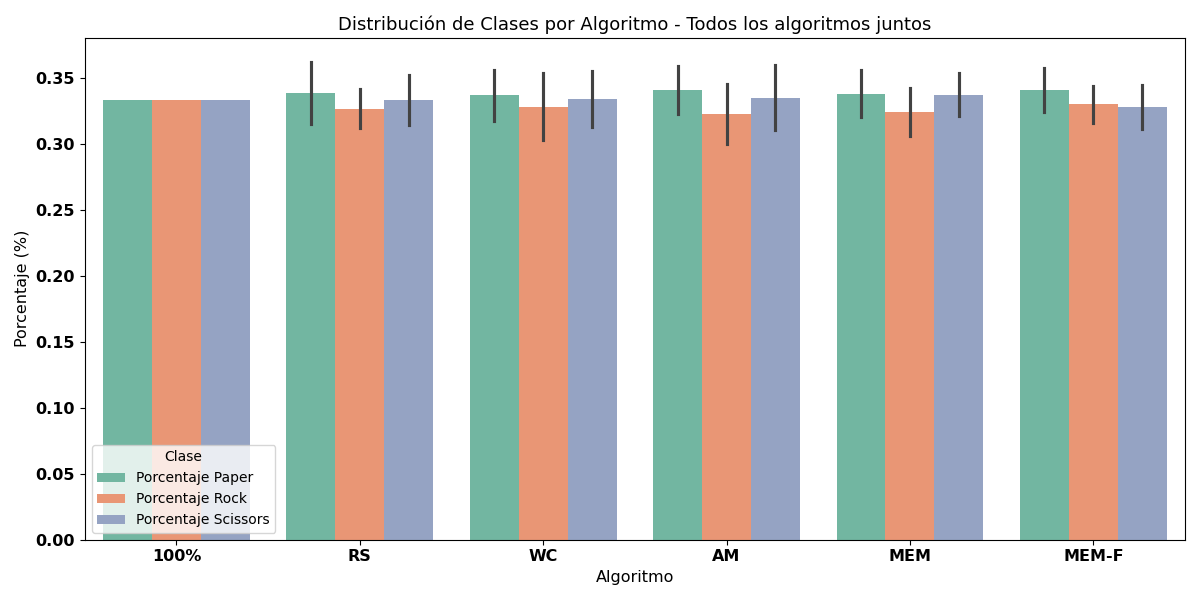
\includegraphics[width=0.95\textwidth]{imagenes/evaluaciones/final/distribucion-de-clases}
    \caption{Distribución de clases seleccionadas por cada algoritmo en el conjunto reducido final.}
    \label{fig:distribucion-de-clases-final}
\end{figure}

El análisis de la distribución de clases en los subconjuntos finales permite evaluar si los algoritmos de reducción mantienen
un equilibrio adecuado entre las diferentes clases presentes en el dataset original.
Como se observa en la Figura~\ref{fig:distribucion-de-clases-final}, todos los algoritmos tienden a preservar un reparto
razonablemente balanceado entre las clases \textit{Paper}, \textit{Rock} y \textit{Scissors}, con porcentajes cercanos al 33\%.

Sin embargo, se aprecian ligeras variaciones en la estabilidad de la distribución según el algoritmo utilizado.
Los algoritmos \texttt{MA} y \texttt{MA-F} presentan una mayor consistencia en el reparto de clases,
mostrando menores desviaciones y barras de error más reducidas.
Esto indica que las soluciones generadas por los enfoques meméticos tienden a conservar de forma más homogénea la diversidad del conjunto original,
evitando la infrarepresentación o sobrecarga de clases específicas.

En contraste, los algoritmos \texttt{RS}, \texttt{GA-WC} y \texttt{GA-AM} muestran una mayor dispersión en los porcentajes de las clases,
especialmente en el caso de \texttt{RS}, lo que refleja una mayor influencia de la aleatoriedad y una menor capacidad para garantizar la estabilidad en la distribución.
Esta variabilidad podría generar sesgos no deseados en el modelo final, afectando su rendimiento en tareas de clasificación.

En resumen, los resultados confirman que los algoritmos meméticos, y en particular \texttt{MA-F},
no solo son eficaces en términos de precisión y reducción de datos, sino que también logran mantener una distribución de clases equilibrada.
Esta propiedad es fundamental para asegurar la generalización del modelo, ya que evita la introducción de desequilibrios que podrían comprometer la calidad del aprendizaje.

\subsection{Síntesis final}\label{sec:sintesis-final}
\begin{table}[htp]
    \centering
    \resizebox{\textwidth}{!}{
        \begin{tabular}{P{2.2cm} P{2cm} P{2cm} P{2cm} P{2cm} P{2cm} P{2cm} P{2cm} P{2cm} P{2.5cm}}
            \toprule
            \textbf{Algoritmo} & \textbf{Duración Total} & \textbf{Duración por Eval.} & \textbf{Accuracy (Avg)} & \textbf{Precision (Avg)} & \textbf{Recall (Avg)} & \textbf{F1-score (Avg)} & \textbf{Evaluaciones} & \textbf{Porc.
            Final}                                                                                                                                                                                                                    \\
            \midrule
            \multicolumn{9}{l}{\textbf{10\%}}                                                                                                                                                                                         \\
            \midrule
            RS                 & 00:38:17                & 00:00:22                    & 81,34\%                 & 82,46\%                  & 81,34\%               & 80,52\%                 & 100                   & 10,00\%       \\
            GA-WC              & 00:34:03                & 00:00:21                    & 83,60\%                 & 84,38\%                  & 83,60\%               & 82,82\%                 & 100                   & 10,00\%       \\
            GA-AM              & 00:27:39                & 00:00:17                    & 83,66\%                 & 84,24\%                  & 83,66\%               & 83,09\%                 & 100                   & 10,00\%       \\
            MA                 & 00:27:43                & 00:00:17                    & 82,85\%                 & 84,44\%                  & 82,85\%               & 81,91\%                 & 100                   & 10,00\%       \\
            MA-F               & 00:32:39                & 00:00:20                    & 83,28\%                 & 84,70\%                  & 83,28\%               & 82,46\%                 & 100                   & 9,62\%        \\
            \midrule
            \multicolumn{9}{l}{\textbf{25\%}}                                                                                                                                                                                         \\
            \midrule
            RS                 & 01:18:22                & 00:00:47                    & 80,70\%                 & 81,90\%                  & 80,70\%               & 79,90\%                 & 100                   & 25,00\%       \\
            GA-WC              & 01:10:21                & 00:00:43                    & 82,37\%                 & 83,86\%                  & 82,37\%               & 81,57\%                 & 100                   & 25,00\%       \\
            GA-AM              & 00:57:29                & 00:00:34                    & 82,42\%                 & 83,68\%                  & 82,42\%               & 81,78\%                 & 100                   & 25,00\%       \\
            MA                 & 00:57:12                & 00:00:34                    & 81,99\%                 & 83,11\%                  & 81,99\%               & 81,21\%                 & 100                   & 25,00\%       \\
            MA-F               & 01:08:54                & 00:00:41                    & 82,80\%                 & 83,77\%                  & 82,80\%               & 82,17\%                 & 100                   & 27,18\%       \\
            \midrule
            \multicolumn{9}{l}{\textbf{50\%}}                                                                                                                                                                                         \\
            \midrule
            RS                 & 02:26:40                & 00:01:28                    & 80,86\%                 & 82,65\%                  & 80,86\%               & 80,22\%                 & 100                   & 50,00\%       \\
            GA-WC              & 02:15:43                & 00:01:21                    & 81,61\%                 & 83,78\%                  & 81,61\%               & 81,06\%                 & 100                   & 50,00\%       \\
            GA-AM              & 01:47:31                & 00:01:05                    & 81,13\%                 & 82,62\%                  & 81,13\%               & 80,41\%                 & 100                   & 50,00\%       \\
            MA                 & 01:47:32                & 00:01:05                    & 81,51\%                 & 83,36\%                  & 81,51\%               & 80,89\%                 & 100                   & 50,00\%       \\
            MA-F               & 02:16:51                & 00:01:22                    & 81,61\%                 & 83,09\%                  & 81,61\%               & 80,96\%                 & 100                   & 67,07\%       \\
            \midrule
            \multicolumn{9}{l}{\textbf{75\%}}                                                                                                                                                                                         \\
            \midrule
            RS                 & 03:05:49                & 00:01:51                    & 82,26\%                 & 84,16\%                  & 82,26\%               & 81,67\%                 & 100                   & 75,00\%       \\
            GA-WC              & 03:33:06                & 00:02:08                    & 82,31\%                 & 83,91\%                  & 82,31\%               & 81,59\%                 & 100                   & 75,00\%       \\
            GA-AM              & 02:36:41                & 00:01:34                    & 82,42\%                 & 83,94\%                  & 82,42\%               & 81,85\%                 & 100                   & 75,00\%       \\
            MA                 & 02:37:43                & 00:01:35                    & 82,74\%                 & 84,33\%                  & 82,74\%               & 82,14\%                 & 100                   & 75,00\%       \\
            MA-F               & 03:08:21                & 00:01:53                    & 82,69\%                 & 84,18\%                  & 82,69\%               & 82,10\%                 & 100                   & 71,16\%       \\
            \midrule
            \multicolumn{9}{l}{\textbf{100\%}}                                                                                                                                                                                        \\
            \midrule
            100\%              & -                       & 00:03:15                    & 78,60\%                 & 81,55\%                  & 78,60\%               & 77,68\%                 & 1                     & 100,00\%      \\
            \bottomrule
        \end{tabular}
    }
    \caption{Resultados detallados por porcentaje inicial y algoritmo: precisión, evaluaciones y duración.}
    \label{tab:resultados-generales-por-porcentaje-inicial}
\end{table}

Los resultados globales obtenidos para el conjunto de datos Rock, Paper, Scissors (véase Tabla~\ref{tab:resultados-generales-por-porcentaje-inicial})
permiten extraer conclusiones claras sobre el rendimiento de los algoritmos evaluados.

En primer lugar, el \texttt{MA-F} se consolida como la solución más robusta y eficaz: no solo alcanza la mayor precisión en términos de \textit{accuracy},
sino que también logra mantener un porcentaje reducido de datos seleccionados, optimizando la eficiencia del modelo sin comprometer su rendimiento.
Además, \texttt{MA-F} presenta una notable estabilidad entre ejecuciones,
reflejada en su baja dispersión y en la conservación de una distribución equilibrada de clases en los subconjuntos generados.
Estos resultados demuestran su capacidad para superar incluso a la referencia del 100\% de datos, logrando un mejor rendimiento con menos instancias.

El \texttt{MA} también ofrece resultados sobresalientes, manteniendo altos niveles de precisión y una considerable reducción de datos.
Sin embargo, presenta una ligera mayor variabilidad en comparación con \texttt{MA-F}, lo que sugiere una estabilidad algo inferior en ciertos escenarios.

Por otro lado, el \texttt{GA-AM} mejora respecto a enfoques más simples como \texttt{RS} y \texttt{GA-WC}, alcanzando resultados intermedios en términos de precisión y reducción de datos.
Sin embargo, no logra superar la consistencia ni la eficiencia de los enfoques meméticos, mostrando una estabilidad moderada en la distribución de clases.

El \texttt{GA-WC} ofrece ligeras mejoras frente a la búsqueda aleatoria,
pero mantiene una mayor dispersión de resultados y requiere porcentajes de datos más elevados para alcanzar precisiones competitivas.
Esto limita su eficacia en escenarios donde la reducción de datos es prioritaria.

Finalmente, la \texttt{RS}, utilizada como referencia, queda claramente superada por todos los enfoques evolutivos y meméticos.
Sus resultados muestran una alta variabilidad, una menor precisión global y una mayor propensión a generar subconjuntos con distribuciones de clases menos estables,
lo que pone de manifiesto la importancia de utilizar estrategias de selección guiada para optimizar tanto el rendimiento como la estabilidad del modelo.

En conjunto, este análisis confirma que los MA, especialmente en su versión libre,
representan la mejor alternativa para abordar la selección de subconjuntos de datos en tareas de aprendizaje profundo.
Logran un equilibrio óptimo entre precisión, eficiencia y estabilidad, superando ampliamente a las técnicas basadas en selección aleatoria o enfoques genéticos más sencillos.


\section{Validación con el dataset \texttt{PAINTING}}\label{sec:validacion-con-painting}
Para comprobar la robustez de los algoritmos desarrollados, se validan los experimentos con el dataset \texttt{PAINTING},
caracterizado por una mayor complejidad visual y un número superior de clases respecto al conjunto \texttt{RPS}.
Con el fin de mantener un equilibrio entre complejidad y coste computacional, se limitan los experimentos a los porcentajes iniciales del 25\% y 50\%,
evaluando únicamente los algoritmos más representativos.

En particular, se selecciona el MA, junto con su versión libre, ya que ambos han demostrado ser los más eficaces en las pruebas anteriores.
Para establecer una referencia clara, se incluyen también los resultados obtenidos usando el 100\% del conjunto de datos, y para la comparación de
\textit{accuracy} entre algoritmos también se añade el resultado del RS.

\subsection{Comparación de \textit{accuracy} entre algoritmos}
\begin{figure}[htp]
    \centering
    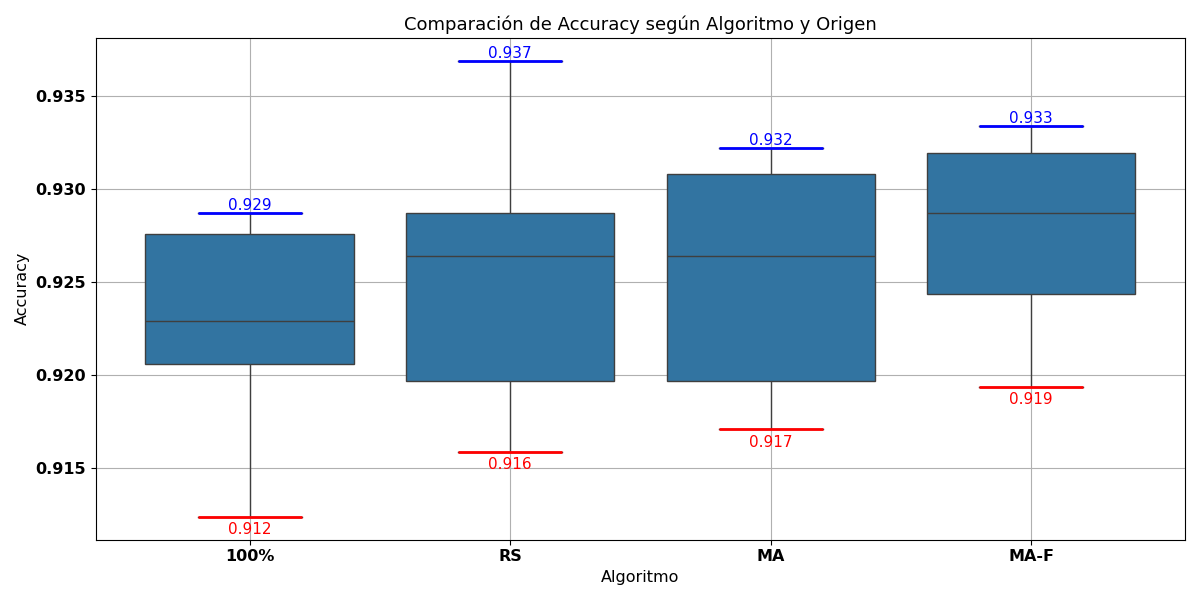
\includegraphics[width=1\textwidth]{imagenes/evaluaciones/painting/comparacion-por-algoritmo}
    \caption{Boxplot comparando resultados con el dataset \texttt{PAINTING} usando \textit{accuracy}.}
    \label{fig:comparacion-por-algoritmo}
\end{figure}

En la Figura~\ref{fig:comparacion-por-algoritmo} se comparan los valores de \textit{accuracy} obtenidos al aplicar distintos
algoritmos de selección de subconjuntos en el conjunto de datos \texttt{PAINTING}.
A simple vista, destaca el buen rendimiento de los tres enfoques meméticos frente al uso directo del 100\% del conjunto o la selección aleatoria,
lo cual es especialmente significativo al tratarse de un conjunto con alta complejidad visual y estructural.

El MA-F obtiene el mejor rendimiento general, con una mediana que ronda el \textbf{0.927} y un valor máximo de \textbf{0.933},
superando incluso la ejecución con el 100\% de los datos, cuyo máximo se sitúa en \textbf{0.929}.
Esto no solo refuerza su capacidad de generalización, sino que demuestra que una selección optimizada puede superar a la totalidad del conjunto original,
posiblemente por eliminar ejemplos redundantes o incluso perjudiciales.

El MA también muestra una precisión elevada, con una mediana apenas inferior al libre, y un máximo de \textbf{0.931}.
Sin embargo, su varianza es ligeramente mayor, lo que sugiere que la falta de ajuste dinámico del tamaño del subconjunto puede limitar su adaptabilidad en ciertas ejecuciones.

Por otro lado, la selección aleatoria, aunque muestra valores aceptables, vuelve a confirmar su principal debilidad: la alta dispersión.
Con un mínimo de \textbf{0.916} y una mediana prácticamente idéntica a la obtenida con el uso completo del dataset,
su comportamiento se sitúa como una referencia básica pero poco fiable.
Puede alcanzar buenos resultados, pero lo hace de forma inconsistente y sin mecanismos que garanticen estabilidad.

La ejecución con el \textbf{100\%} de los datos, utilizada como referencia absoluta, queda por debajo de las soluciones obtenidas por los algoritmos meméticos.
Esto valida empíricamente que no es la cantidad de datos, sino su calidad y representatividad, lo que determina la eficacia del entrenamiento en entornos complejos.

% \colorbox{yellow}{¿Añadir el párrafo de resumen?}
% En conjunto, esta comparación deja clara la superioridad de las estrategias meméticas, especialmente en su versión libre,
% tanto por su rendimiento medio como por su estabilidad.
% Esto refuerza la hipótesis de que los algoritmos de selección basados en evolución y búsqueda local son capaces de generar
% subconjuntos más eficientes y fiables que los enfoques ingenuos o el uso total de los datos.
En resumen, los algoritmos meméticos, especialmente en su versión libre, muestran el mejor rendimiento en términos de precisión y estabilidad,
superando al uso del 100\% de los datos y al enfoque aleatorio.

\subsection{Impacto del porcentaje inicial}
\begin{figure}[htp]
    \centering
    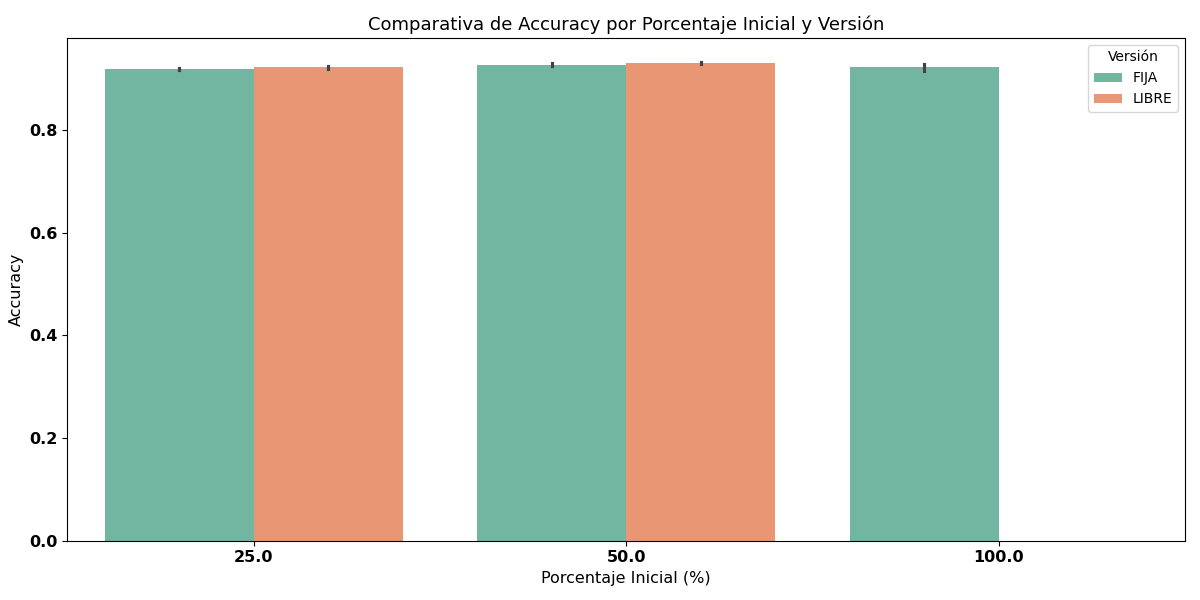
\includegraphics[width=1\textwidth]{imagenes/evaluaciones/painting/comparacion-por-porcentaje}
    \caption{Diagrama de barras de \textit{accuracy} según el porcentaje inicial de datos del MA, MA-F y el 100\%.}
    \label{fig:accuracy_porcentaje_painting}
\end{figure}

\begin{figure}[htp]
    \centering
    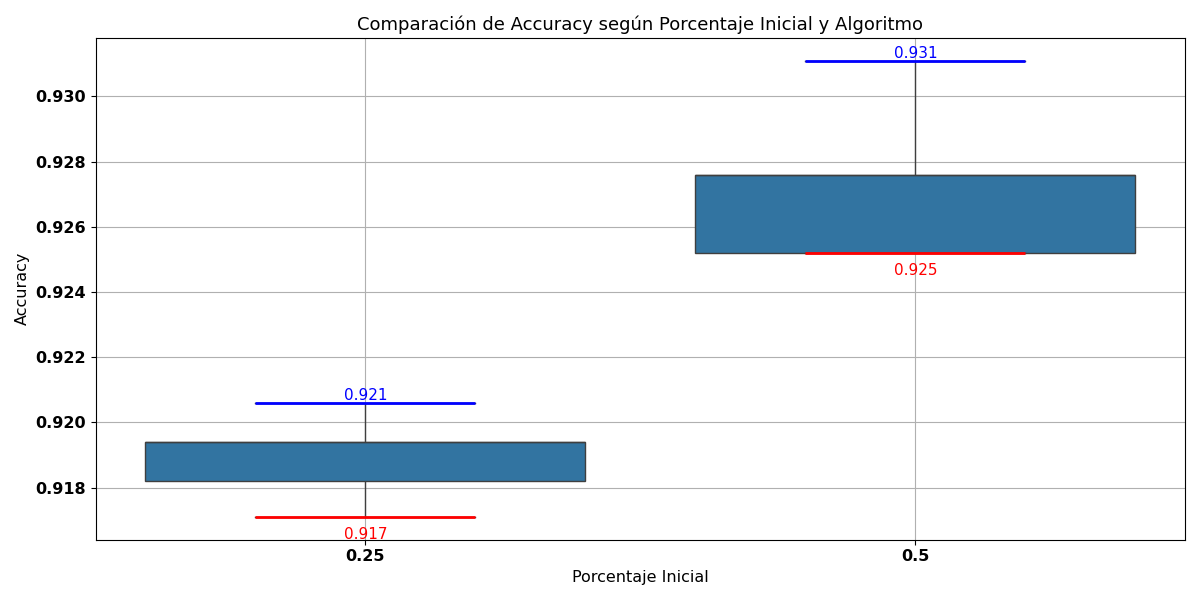
\includegraphics[width=1\textwidth]{imagenes/evaluaciones/painting/comparacion-por-porcentaje-mem}
    \caption{Boxplot de \textit{accuracy} para el algoritmo memético (\texttt{MA}) según el porcentaje inicial de datos en el dataset \texttt{PAINTING}.}
    \label{fig:comparacion-por-porcentaje-mem}
\end{figure}

\begin{figure}[htp]
    \centering
    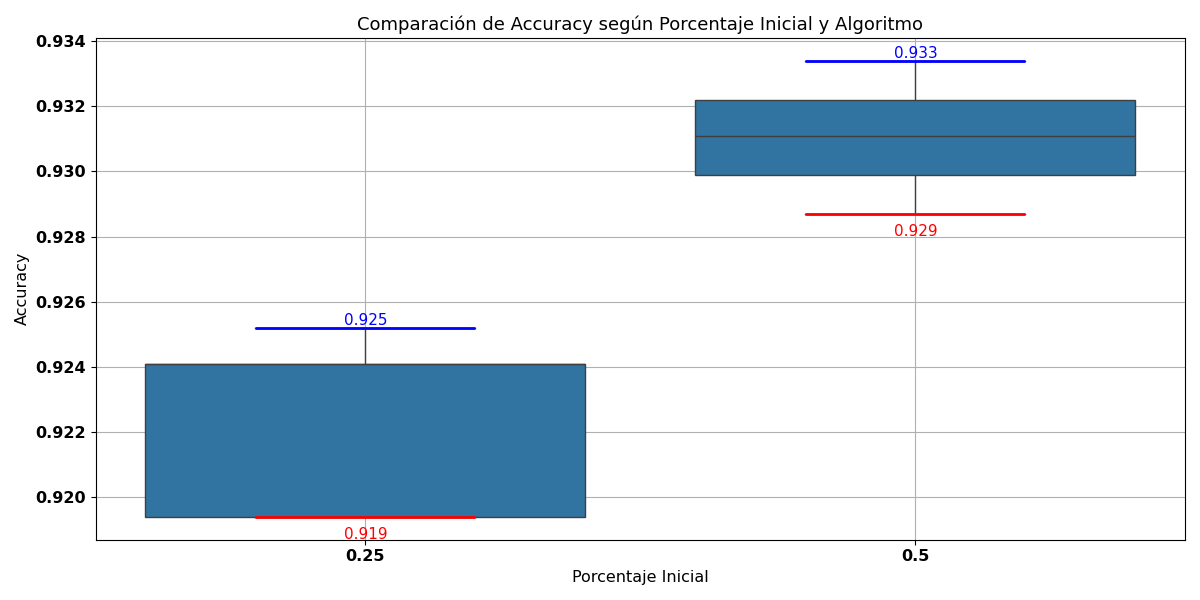
\includegraphics[width=1\textwidth]{imagenes/evaluaciones/painting/comparacion-por-porcentaje-mem-f}
    \caption{Boxplot de \textit{accuracy} para el algoritmo memético libre (\texttt{MA-F}) según el porcentaje inicial de datos en el dataset \texttt{PAINTING}.}
    \label{fig:comparacion-por-porcentaje-mem-f}
\end{figure}

\begin{table}[htp]
    \centering
    \resizebox{\textwidth}{!}{
        \begin{tabular}{P{2.5cm} P{2cm} P{2.5cm} P{2.5cm} P{2.5cm} P{2.5cm} P{2cm}}
            \toprule
            \textbf{Algoritmo} & \textbf{Accuracy (Avg)} & \textbf{Precision (Avg)} & \textbf{Recall (Avg)} & \textbf{F1-score (Avg)} & \textbf{Evaluaciones} & \textbf{Porc.
            Final}                                                                                                                                                            \\
            \midrule
            \multicolumn{7}{l}{\textbf{25\%}}                                                                                                                                 \\
            \midrule
            MA                 & 91,89\%                 & 91,63\%                  & 91,89\%               & 91,67\%                 & 100                   & 25,00\%       \\
            MA-F               & 92,24\%                 & 92,06\%                  & 92,24\%               & 92,09\%                 & 100                   & 41,35\%       \\
            \midrule
            \multicolumn{7}{l}{\textbf{50\%}}                                                                                                                                 \\
            \midrule
            MA                 & 92,73\%                 & 92,61\%                  & 92,73\%               & 92,63\%                 & 100                   & 50,00\%       \\
            MA-F               & 93,11\%                 & 93,00\%                  & 93,11\%               & 93,01\%                 & 100                   & 68,69\%       \\
            \midrule
            \multicolumn{7}{l}{\textbf{100\%}}                                                                                                                                \\
            \midrule
            100\%              & 92,24\%                 & 92,05\%                  & 92,24\%               & 92,06\%                 & 1                     & 100,00\%      \\
            \bottomrule
        \end{tabular}
    }
    \caption{Resultados de los algoritmos meméticos y uso del 100\% en el dataset \texttt{PAINTING}.}
    \label{tab:resultados-memetico-painting}
\end{table}

\colorbox{yellow}{FALTA añadir los resultados del 75\%.}


\colorbox{yellow}{FALTA ajustar mejor el analisis.}

La Figura~\ref{fig:accuracy_porcentaje_painting} muestra cómo varía el rendimiento del modelo (medido en términos de \textit{accuracy})
al utilizar diferentes porcentajes iniciales de datos para los algoritmos meméticos en el dataset \texttt{PAINTING}.
Lo primero que destaca es que el uso del 50\% del conjunto original no solo logra un rendimiento equiparable, sino incluso superior al uso del 100\%.
Con una mediana cercana a \textbf{0.930} y un máximo de \textbf{0.933}, este porcentaje logra un equilibrio ideal entre compresión de datos y preservación de información relevante.

Este resultado sugiere que, a partir de cierto umbral, añadir más datos no solo deja de aportar valor, sino que puede introducir ruido o redundancia.
En este caso, el entrenamiento con el 100\% de los datos exhibe mayor dispersión y un mínimo significativamente más bajo (\textbf{0.912}),
lo cual indica una mayor variabilidad entre ejecuciones y una menor estabilidad general.

Por otro lado, el uso del 25\% inicial también demuestra un rendimiento sorprendentemente competitivo,
alcanzando un máximo de \textbf{0.925}.
Sin embargo, su rango intercuartílico más estrecho (menor dispersión de los resultados) y su menor valor mínimo
(\textbf{0.917}) evidencian una cierta fragilidad ante la reducción excesiva:
puede funcionar bien si la selección es óptima, pero el margen de error es menor.

Este comportamiento ilustra un fenómeno interesante en la reducción de datos: no existe una relación lineal entre cantidad de datos y precisión,
sino que el valor está en la calidad y representatividad del subconjunto.
El resultado más robusto refuerza la hipótesis de que existe un punto de saturación
a partir del cual la adición de ejemplos tiene un efecto marginal o incluso contraproducente en modelos convolucionales.

% \colorbox{yellow}{¿Añadir el párrafo de resumen?}
% En conjunto, los resultados de este apartado respaldan la viabilidad de aplicar técnicas de reducción de datos en entornos reales,
% sugiriendo que con solo la mitad de los datos cuidadosamente seleccionados se puede no solo igualar,
% sino superar el rendimiento de un entrenamiento exhaustivo con todo el dataset.
En resumen, los resultados respaldan la viabilidad de utilizar una fracción cuidadosamente seleccionada de datos para obtener
resultados comparables o incluso superiores al uso del conjunto completo.

\subsection{Equilibrio en la distribución de clases}
\begin{figure}[htp]
    \centering
    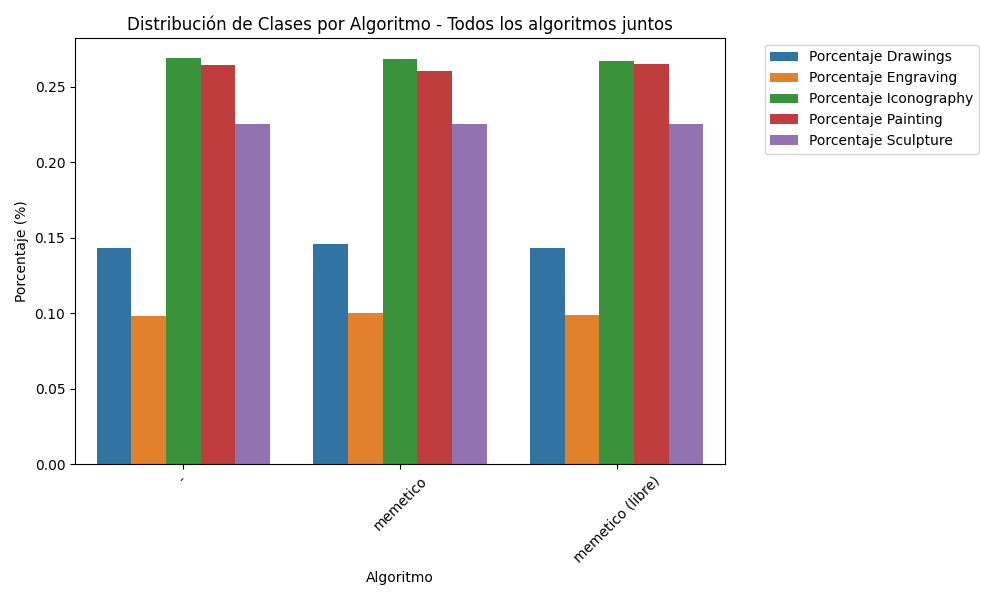
\includegraphics[width=0.9\textwidth]{imagenes/evaluaciones/painting/balance-de-clases-por-algoritmo}
    \caption{Distribución de clases seleccionadas por cada algoritmo.}
    \label{fig:balance_clases_painting}
\end{figure}

La Figura~\ref{fig:balance_clases_painting} muestra la proporción de clases preservada por cada algoritmo durante el proceso de reducción.
Se observa que tanto el MA como el MA-F mantienen una distribución prácticamente idéntica a la original,
sin introducir sesgos estructurales.

Las clases mayoritarias (\texttt{Iconography}, \texttt{Painting} y \texttt{Sculpture}) se mantienen consistentes en su proporción,
al igual que las clases minoritarias (\texttt{Drawings} y \texttt{Engraving}).
Esta conservación sugiere que el proceso de selección no actúa de forma aleatoria ni ciega,
sino que incorpora implícitamente una presión hacia la diversidad, lo cual es clave en problemas multiclase.

\subsection{Evolución del tamaño del subconjunto}
\begin{figure}[htp]
    \centering
    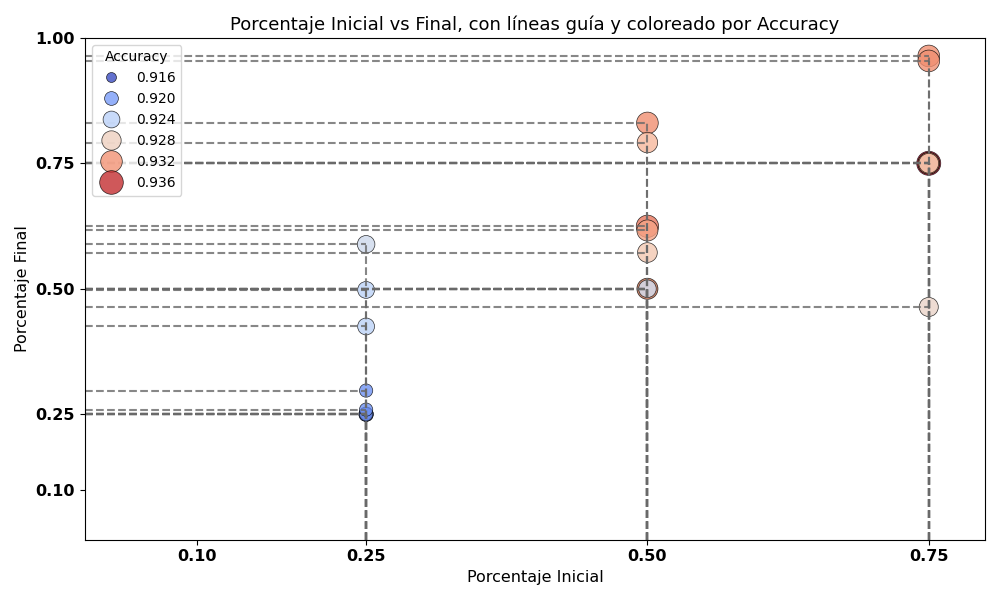
\includegraphics[width=0.9\textwidth]{imagenes/evaluaciones/painting/scatter-por-porcentaje}
    \caption{Evolución del tamaño del subconjunto seleccionado por los algoritmos libres según el porcentaje inicial.}
    \label{fig:evolucion_porcentaje_libre}
\end{figure}

\colorbox{yellow}{Volver a mencionar la tabla de resultados.}

En la Figura~\ref{fig:evolucion_porcentaje_libre} se analiza cómo evoluciona el tamaño de los subconjuntos seleccionados por los algoritmos libres respecto al valor inicial.
Se observa que el MA-F tiende a incrementar el porcentaje de imágenes seleccionadas durante el proceso evolutivo.

Este comportamiento adaptativo pone de manifiesto la capacidad del algoritmo para ajustar dinámicamente la escala de la solución en función de la complejidad del problema.
A diferencia de enfoques con tamaño fijo, el algoritmo libre no solo decide qué ejemplos seleccionar, sino también cuántos,
ampliando el conjunto cuando detecta que puede mejorar el rendimiento sin incurrir en sobreajuste.

Además, se observa que al partir del 25\% inicial, el algoritmo tiende a aumentar el tamaño del subconjunto hasta un 16,35\% adicional,
en cambio, al partir del 50\% inicial, el crecimiento es mayor, alcanzando un 18,69\% adicional.
Este hecho puede sugerir una cierta prudencia evolutiva: el algoritmo no se expande indiscriminadamente,
sino que responde a señales de mejora en el proceso de evaluación.
Este mecanismo emergente refuerza la versatilidad del enfoque libre, que no solo busca soluciones de alta calidad,
sino que lo hace optimizando también el volumen de datos utilizados.


\bigskip

\subsection*{Síntesis final de la validación con \texttt{PAINTING}}
Los resultados obtenidos con el dataset \texttt{PAINTING} confirman la solidez y capacidad de generalización de los algoritmos desarrollados.
Tanto el enfoque memético estándar como, especialmente, su versión libre, lograron mantener un rendimiento competitivo en un entorno más complejo y con mayor número de clases.

Se evidencia que es posible superar el rendimiento del conjunto completo de entrenamiento utilizando únicamente un subconjunto bien seleccionado,
reduciendo significativamente el volumen de datos sin comprometer la precisión.
Además, los algoritmos meméticos demuestra preservar el equilibrio entre clases y adaptarse dinámicamente al tamaño del subconjunto,
lo que constituye una ventaja clave en tareas reales donde no siempre se dispone de datasets perfectamente balanceados ni completos.

En conjunto, esta validación externa no solo refuerza las conclusiones obtenidas con \texttt{RPS},
sino que demuestra que el uso de técnicas evolutivas, y en particular las variantes libres, puede ser una alternativa eficaz,
escalable y controlable frente a la selección masiva o aleatoria de datos en procesos de entrenamiento profundo.
